\documentclass[12pt,a4paper]{article}

% ── Packages ──
\usepackage[utf8]{inputenc}
\usepackage[T1]{fontenc}
\usepackage{lmodern}
\usepackage[margin=1in]{geometry}
\usepackage{amsmath,amssymb,amsthm}
\usepackage{graphicx}
\usepackage{booktabs}
\usepackage{float}
\usepackage{caption}
\usepackage{subcaption}
\usepackage{hyperref}
\usepackage{enumitem}
\usepackage{xcolor}
\usepackage{array}
\usepackage{tabularx}
\usepackage{algorithm}
\usepackage{algpseudocode}
\usepackage{multirow}

\hypersetup{
    colorlinks=true,
    linkcolor=blue!60!black,
    citecolor=green!50!black,
    urlcolor=blue!70!black,
}

\newtheorem{definition}{Definition}
\newtheorem{proposition}{Proposition}

\title{%
    \textbf{Product-Level Markdown Pricing Simulator} \\[6pt]
    \large A Multi-Model Demand Estimation and MDP-Based \\
    Discount Optimization Framework \\[6pt]
    \normalsize Applied to the Dunnhumby Complete Journey Dataset
}
\author{Pricing Analytics Research}
\date{\today}

\begin{document}
\maketitle

\begin{abstract}
We develop a product-level markdown pricing simulator grounded in a
Markov Decision Process (MDP) formulation where the state vector
encodes per-item selection, discount depth, realized demand, and
cumulative budget consumption, while the action space specifies new
selection and discount vectors across all products. Using the
Dunnhumby Complete Journey dataset (2.6M transactions, 92,339
products, 102 weeks), we estimate individual demand models for 150
representative products selected via stratified revenue-tercile
sampling from 12 data-driven segments (11 of which are represented
in the final selection). We compare five demand model
families---log-log OLS with AR(1) demand persistence, within-segment
cross-product substitution, seasonality, and continuous promotional
controls; Random Forest; XGBoost; LightGBM; and neural
networks---finding that the log-log OLS achieves the strongest lift
correlation ($r = 0.694$) among structurally compatible models.
The demand transition is no longer memoryless: lagged log-demand
enters via an AR(1) persistence term ($\hat{\rho}_i$, 64 products
with $\hat{\rho}_i > 0$ after shrinkage, mean $= 0.039$), and
within-segment cross-product substitution ($\hat{\lambda}_i$, 80
products with $\hat{\lambda}_i < 0$ after shrinkage, mean $=
-0.852$) captures promotional cannibalization. Integration of
promotional causal data (display and mailer exposure from 36.8M
store-product-week records) as continuous exposure fractions yields
37 significant display effects (mean $+1.716$ log-demand) and 29
significant mailer effects (mean $+0.562$ log-demand).
James--Stein empirical Bayes shrinkage with parameter-specific
standard errors toward segment medians regularizes noisy per-product
estimates, applied to elasticities, discount effects, demand
persistence, substitution effects, display effects, and mailer
effects. The calibrated simulator identifies a targeted discount
policy (top-30 by promotional response) that improves revenue by
41.3\% over the no-discount baseline, with Monte Carlo confidence
intervals over 50 replications. Per-product sensitivity analysis
using simulator-based rollouts reveals that 64.7\% of products
benefit from discounting, with a median revenue uplift of 105.1\%
(IQR: 36.8\%--288.8\%).
\end{abstract}

\tableofcontents
\newpage

%% ═══════════════════════════════════════════════════════════
\section{Introduction}
\label{sec:intro}
%% ═══════════════════════════════════════════════════════════

Markdown pricing---the practice of reducing prices on products over
their selling season---is one of the most consequential levers in
retail revenue management. Retailers frequently rely on heuristic
discount rules (e.g., uniform 20\% off) that ignore heterogeneity in
price elasticity and promotional response across products. A principled
approach requires three ingredients: (i)~accurate demand models that
capture how individual product sales respond to price changes and
promotional activity, (ii)~a simulation environment that faithfully
represents the sequential nature of markdown decisions under budget
constraints, and (iii)~a policy evaluation framework that compares
alternative discount strategies.

This work addresses all three requirements. We begin with a thorough
exploratory analysis of the Dunnhumby Complete Journey dataset---a
publicly available retail panel covering 2,500 households, 92,339
products, and 102 weeks of transactions. We then estimate individual
demand functions for 150 representative products using five distinct
model families, ranging from classical econometric specifications to
modern machine learning methods. The estimated demand models feed a
product-level MDP simulator whose state and action spaces operate at
the individual item level, not at the category or segment level.

\subsection{Related Work}

\paragraph{Price Elasticity Estimation.}
The meta-analysis by Bijmolt et~al.\ (2005) consolidates findings
from 1,851 elasticity estimates across 81 studies. They report a mean
price elasticity of $-2.62$ with substantial heterogeneity driven by
product category, brand loyalty, and promotional context. Tellis
(1988) emphasizes the importance of controlling for promotional
variables when estimating price elasticities, as failure to do so
conflates price and promotional effects. Our approach controls for
display placement, mailer inclusion, coupon availability, and
seasonal demand patterns.

\paragraph{Promotional Response Modeling.}
Blattberg and Neslin (1990) provide the foundational framework for
decomposing promotional effects into price reduction, display,
feature advertising, and coupon components. Van Heerde et~al.\ (2004)
develop decomposition models that separate ``brand switching,''
``purchase acceleration,'' and ``stockpiling'' effects of promotions.
We incorporate display and mailer exposure from the Dunnhumby causal
dataset, which provides store-level promotional indicators for 36.8M
observations.

\paragraph{Markdown Optimization.}
Phillips (2005) and Talluri and van Ryzin (2004) establish the
theoretical foundations for markdown pricing as a dynamic programming
problem. Ferreira et~al.\ (2016) develop an analytics-driven approach
for online retail pricing using demand learning and price optimization.
Our MDP formulation follows the standard framework with per-product
state tracking and budget constraints.

\paragraph{Demand Forecasting with Machine Learning.}
Ban and Rudin (2019) demonstrate that data-driven newsvendor
approaches using tree-based models can outperform parametric methods.
However, for the per-product estimation setting with limited
observations (median 61 weeks per product), we find that classical
log-linear models provide more structurally interpretable parameters
for simulation than flexible tree-based alternatives, which must be
collapsed to two-parameter summaries via finite differences.

%% ═══════════════════════════════════════════════════════════
\section{Data}
\label{sec:data}
%% ═══════════════════════════════════════════════════════════

\subsection{Dataset Overview}

The Dunnhumby ``Complete Journey'' dataset contains two years of
household-level transaction data from a major US grocery retailer.
Table~\ref{tab:data-summary} summarizes the key data files.

\begin{table}[H]
\centering
\caption{Dunnhumby Complete Journey dataset summary.}
\label{tab:data-summary}
\begin{tabular}{lrp{6cm}}
\toprule
\textbf{File} & \textbf{Records} & \textbf{Description} \\
\midrule
transaction\_data & 2,595,732 & Household-product-day transactions
with price, quantity, and discount fields \\
product & 92,339 & Product master with department, commodity, and
brand \\
hh\_demographic & 801 & Household demographics (income, size, age) \\
causal\_data & 36,817,025 & Store-product-week promotional
indicators (display, mailer) \\
coupon & 124,548 & Coupon-product associations \\
coupon\_redempt & 2,318 & Coupon redemption records \\
campaign\_table & 7,207 & Household-campaign associations \\
campaign\_desc & 30 & Campaign descriptions and timing \\
\bottomrule
\end{tabular}
\end{table}

\subsection{Transaction Data Structure}

Each row in the transaction data represents a single household's
purchase of a product on a given day. The key fields and how we use
them are:

\begin{itemize}[nosep]
\item \textbf{SALES\_VALUE}: the dollar amount the customer actually
paid. This is the \emph{net} price after all discounts.

\item \textbf{QUANTITY}: number of units purchased in the transaction.

\item \textbf{RETAIL\_DISC}: the retailer-initiated discount (store
promotion, yellow tag, etc.). Stored as a negative value in the raw
data; we convert to absolute value.

\item \textbf{COUPON\_DISC}: manufacturer or retailer coupon discount.
Also converted to absolute value.

\item \textbf{COUPON\_MATCH\_DISC}: additional coupon-matching
discount provided by the retailer when a manufacturer coupon is
redeemed. Also converted to absolute value.

\item \textbf{WEEK\_NO}: nominal week number (1--102) used as the
temporal index.
\end{itemize}

From these fields, we derive two critical pricing variables. The
total discount combines all three discount components:
\begin{equation}
\label{eq:total-discount}
\text{total\_discount}_j = |\text{RETAIL\_DISC}_j|
+ |\text{COUPON\_DISC}_j| + |\text{COUPON\_MATCH\_DISC}_j|
\end{equation}

The shelf price and discount depth are then:
\begin{align}
\text{shelf\_price}_j &= \frac{\text{SALES\_VALUE}_j +
\text{total\_discount}_j}
{\max(\text{QUANTITY}_j, 1)}
\label{eq:shelf-price}
\\[4pt]
\text{discount\_depth}_j &= \frac{\text{total\_discount}_j}
{\text{SALES\_VALUE}_j + \text{total\_discount}_j}
\label{eq:discount-depth}
\end{align}

The shelf price in Eq.~\eqref{eq:shelf-price} is the
\emph{pre-discount list price per unit}. It reflects what the product
would cost at its normal, undiscounted price. Including
COUPON\_MATCH\_DISC in the total discount ensures that the
reconstructed shelf price and discount depth account for all forms
of price reduction the consumer received.

The discount depth in
Eq.~\eqref{eq:discount-depth} is the fraction of the shelf price
that was forgone due to any form of discount. A transaction
with $\text{discount\_depth} = 0.20$ means the customer paid 80\% of
the shelf price. This separation is fundamental: \emph{shelf price}
captures structural pricing decisions, while \emph{discount depth}
captures promotional activity.

\subsection{Causal Data: Promotional Exposure}

The causal data file records, for each store--product--week
combination, whether a product was on in-store display and/or
included in a mailer advertisement. This file contains
\textbf{36.8 million records} at the store--product--week
granularity.

\begin{itemize}[nosep]
\item \textbf{display}: coded as $0$ (not on display) or positive
integer (type of display). We binarize at the store level:
$\text{on\_display} = \mathbbm{1}[\text{display} \neq 0]$.

\item \textbf{mailer}: coded as letter indicators. We identify
\texttt{A} as mailer inclusion:
$\text{on\_mailer} = \mathbbm{1}[\text{mailer} = \texttt{A}]$.
\end{itemize}

Since the transaction panel is at the product-week level (aggregated
across stores), we aggregate the store-level causal indicators to
product-week by computing the \emph{fraction of stores} where the
product had display/mailer exposure:
\begin{align}
\text{display\_pct}_{it} &= \frac{\text{stores with display for
product } i \text{ in week } t}
{\text{total stores carrying product } i \text{ in week } t}
\end{align}
Unlike earlier iterations that collapsed these fractions to binary
indicators, we use the continuous fractions $\text{display\_pct}_{it}$
and $\text{mailer\_pct}_{it}$ directly in all demand models. This
preserves the intensity of promotional exposure: a product displayed
in 1 out of 100 stores receives a proportionally smaller effect than
one displayed in all stores.

\subsection{Coupon Data}

The coupon file maps 124,548 coupon--product associations from direct
marketing campaigns to specific products. We create a binary flag
$\text{has\_coupon}_i$ indicating whether product $i$ has \emph{any}
associated coupon in the dataset. In our estimation panel, 58.9\% of
product-week observations involve coupon-eligible products.

\subsection{Exploratory Analysis}

The transaction data spans 102 weeks (approximately 2 years). After
filtering to the ``stable period'' (weeks 18--102, excluding initial
ramp-up), we observe consistent weekly patterns in both revenue and
transaction volume.

\begin{figure}[H]
\centering
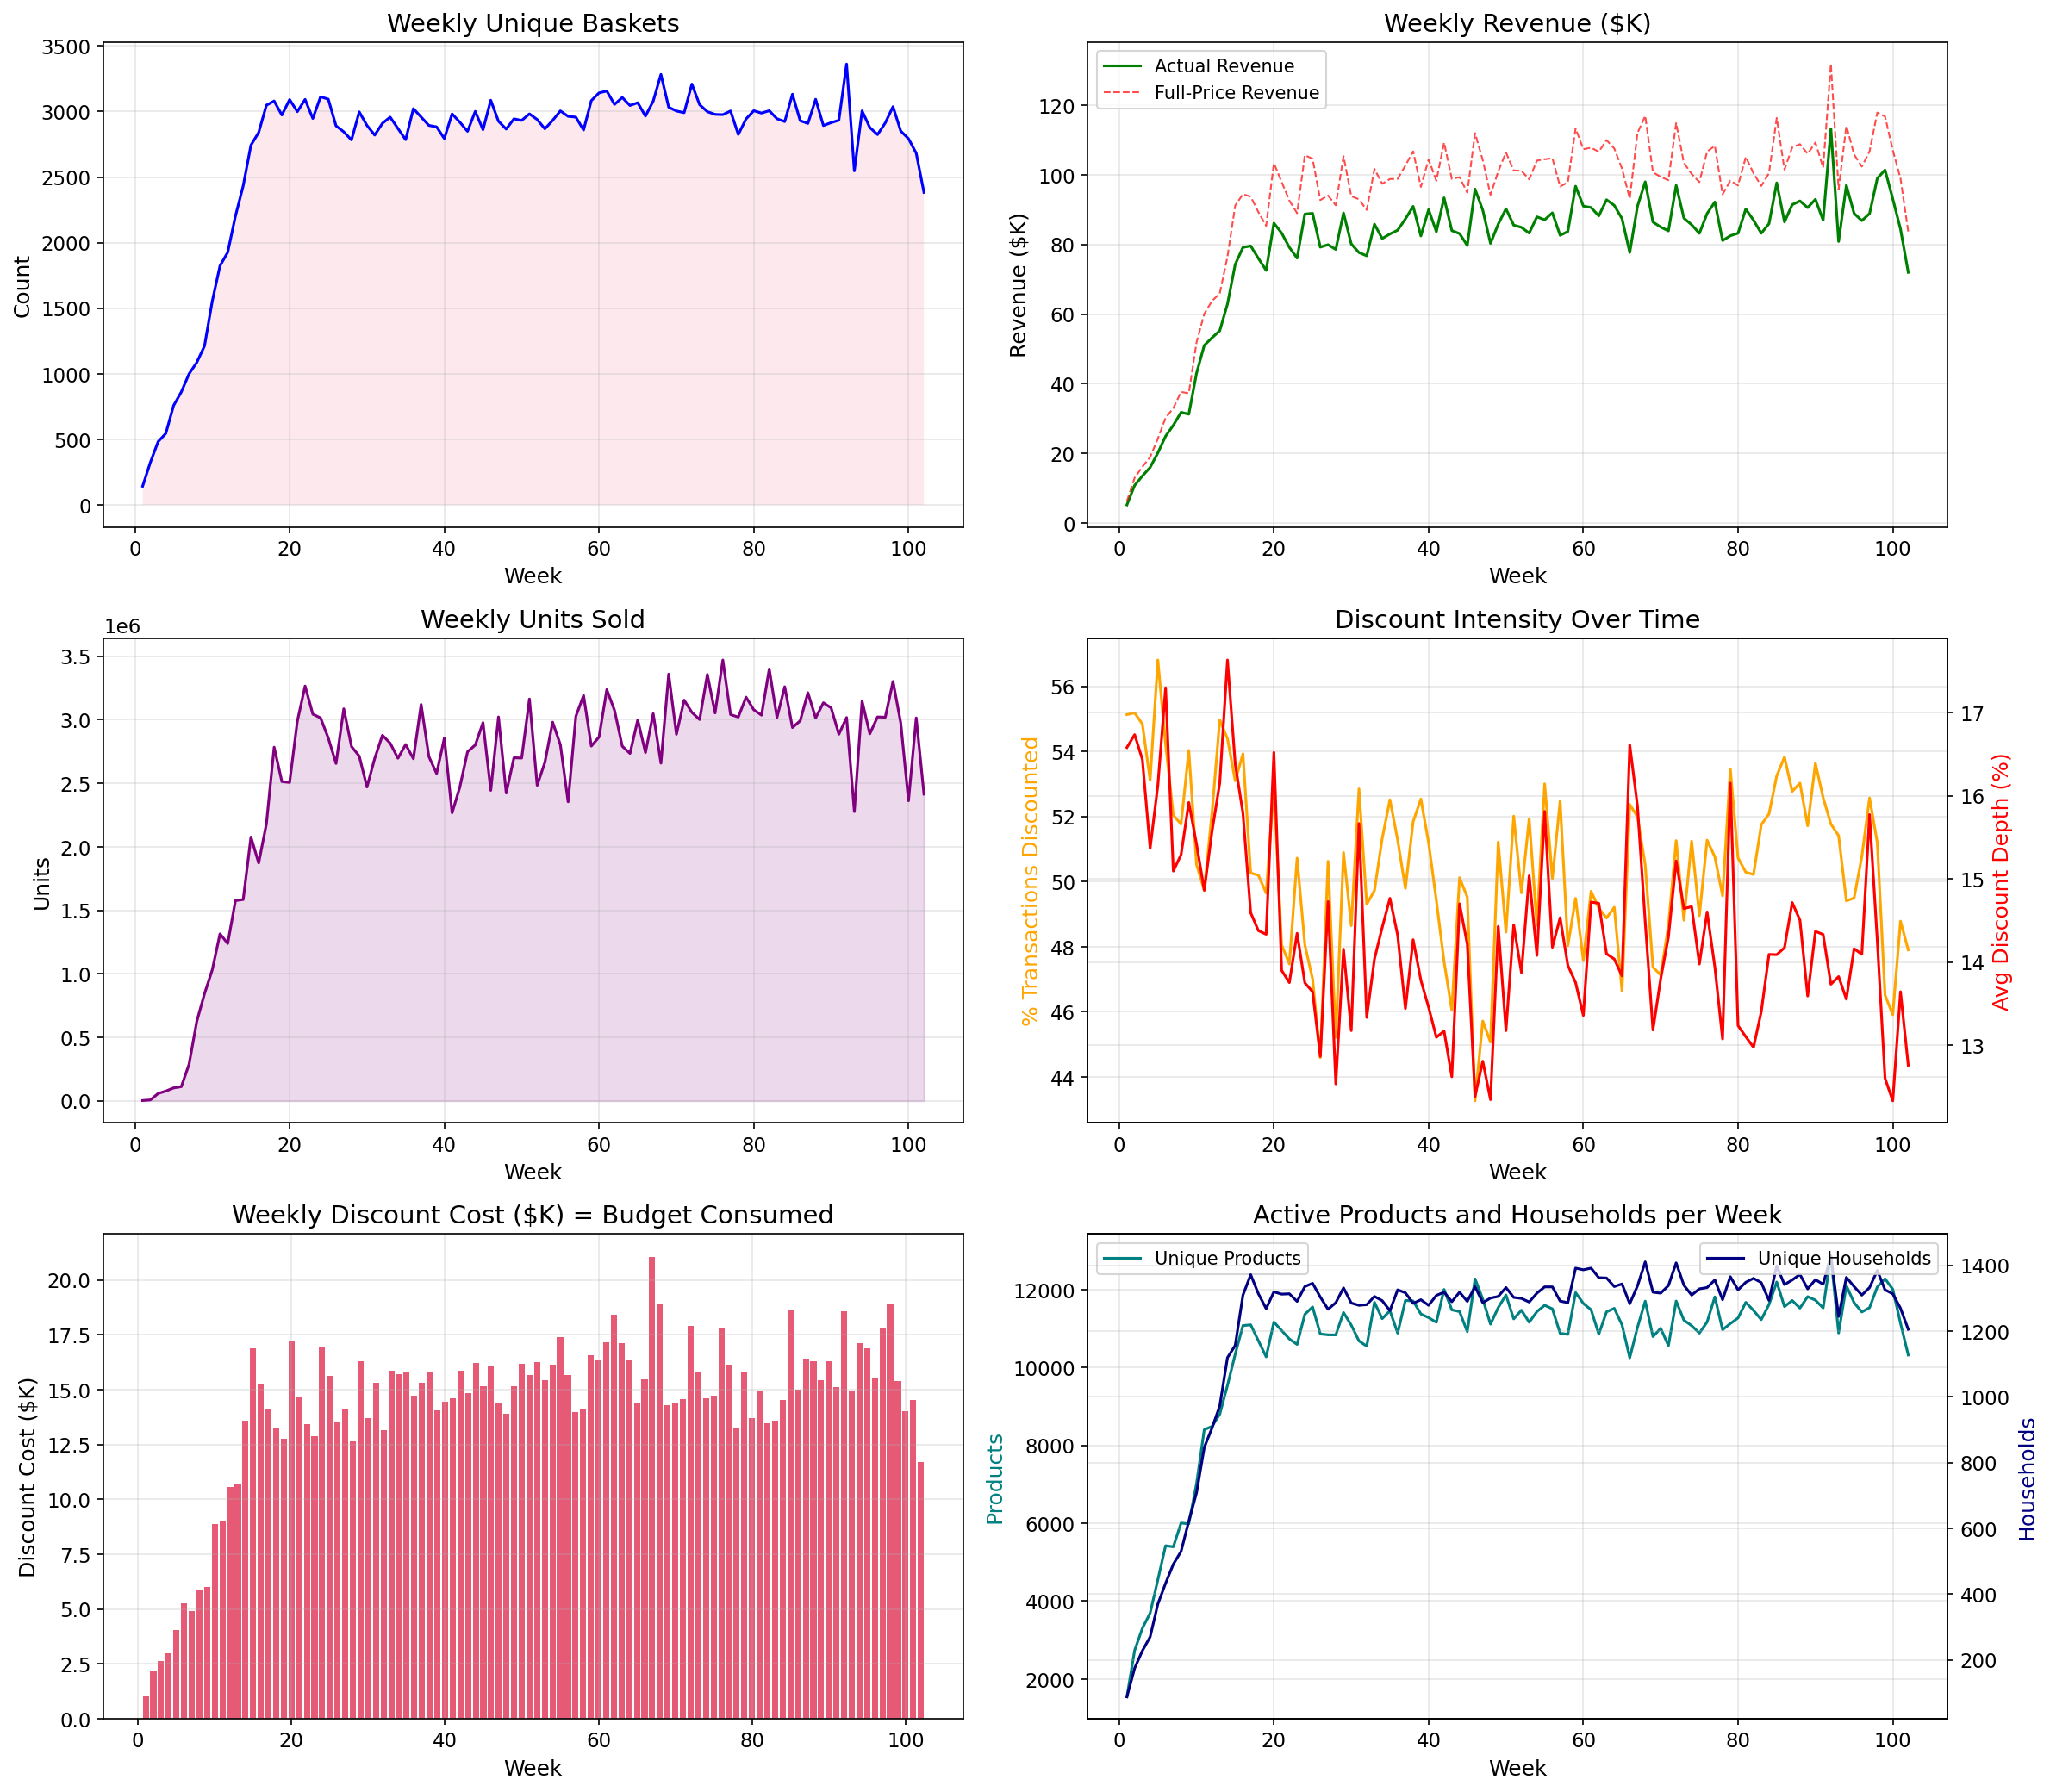
\includegraphics[width=\textwidth]{figures/01_time_series_overview.png}
\caption{Weekly revenue and transaction volume time series showing
stable patterns after week 18 with periodic promotional spikes.}
\label{fig:time-series}
\end{figure}

\paragraph{Price and Discount Patterns.}
Across all transactions, 50.2\% involve some form of retail discount.
Among discounted transactions, the mean discount depth is 26.9\%.
The distribution of discount depths is bimodal, with peaks at
10--15\% (moderate promotions) and 30--40\% (deep clearance
markdowns). This bimodality suggests two distinct promotional
regimes operating in the data.

\begin{figure}[H]
\centering
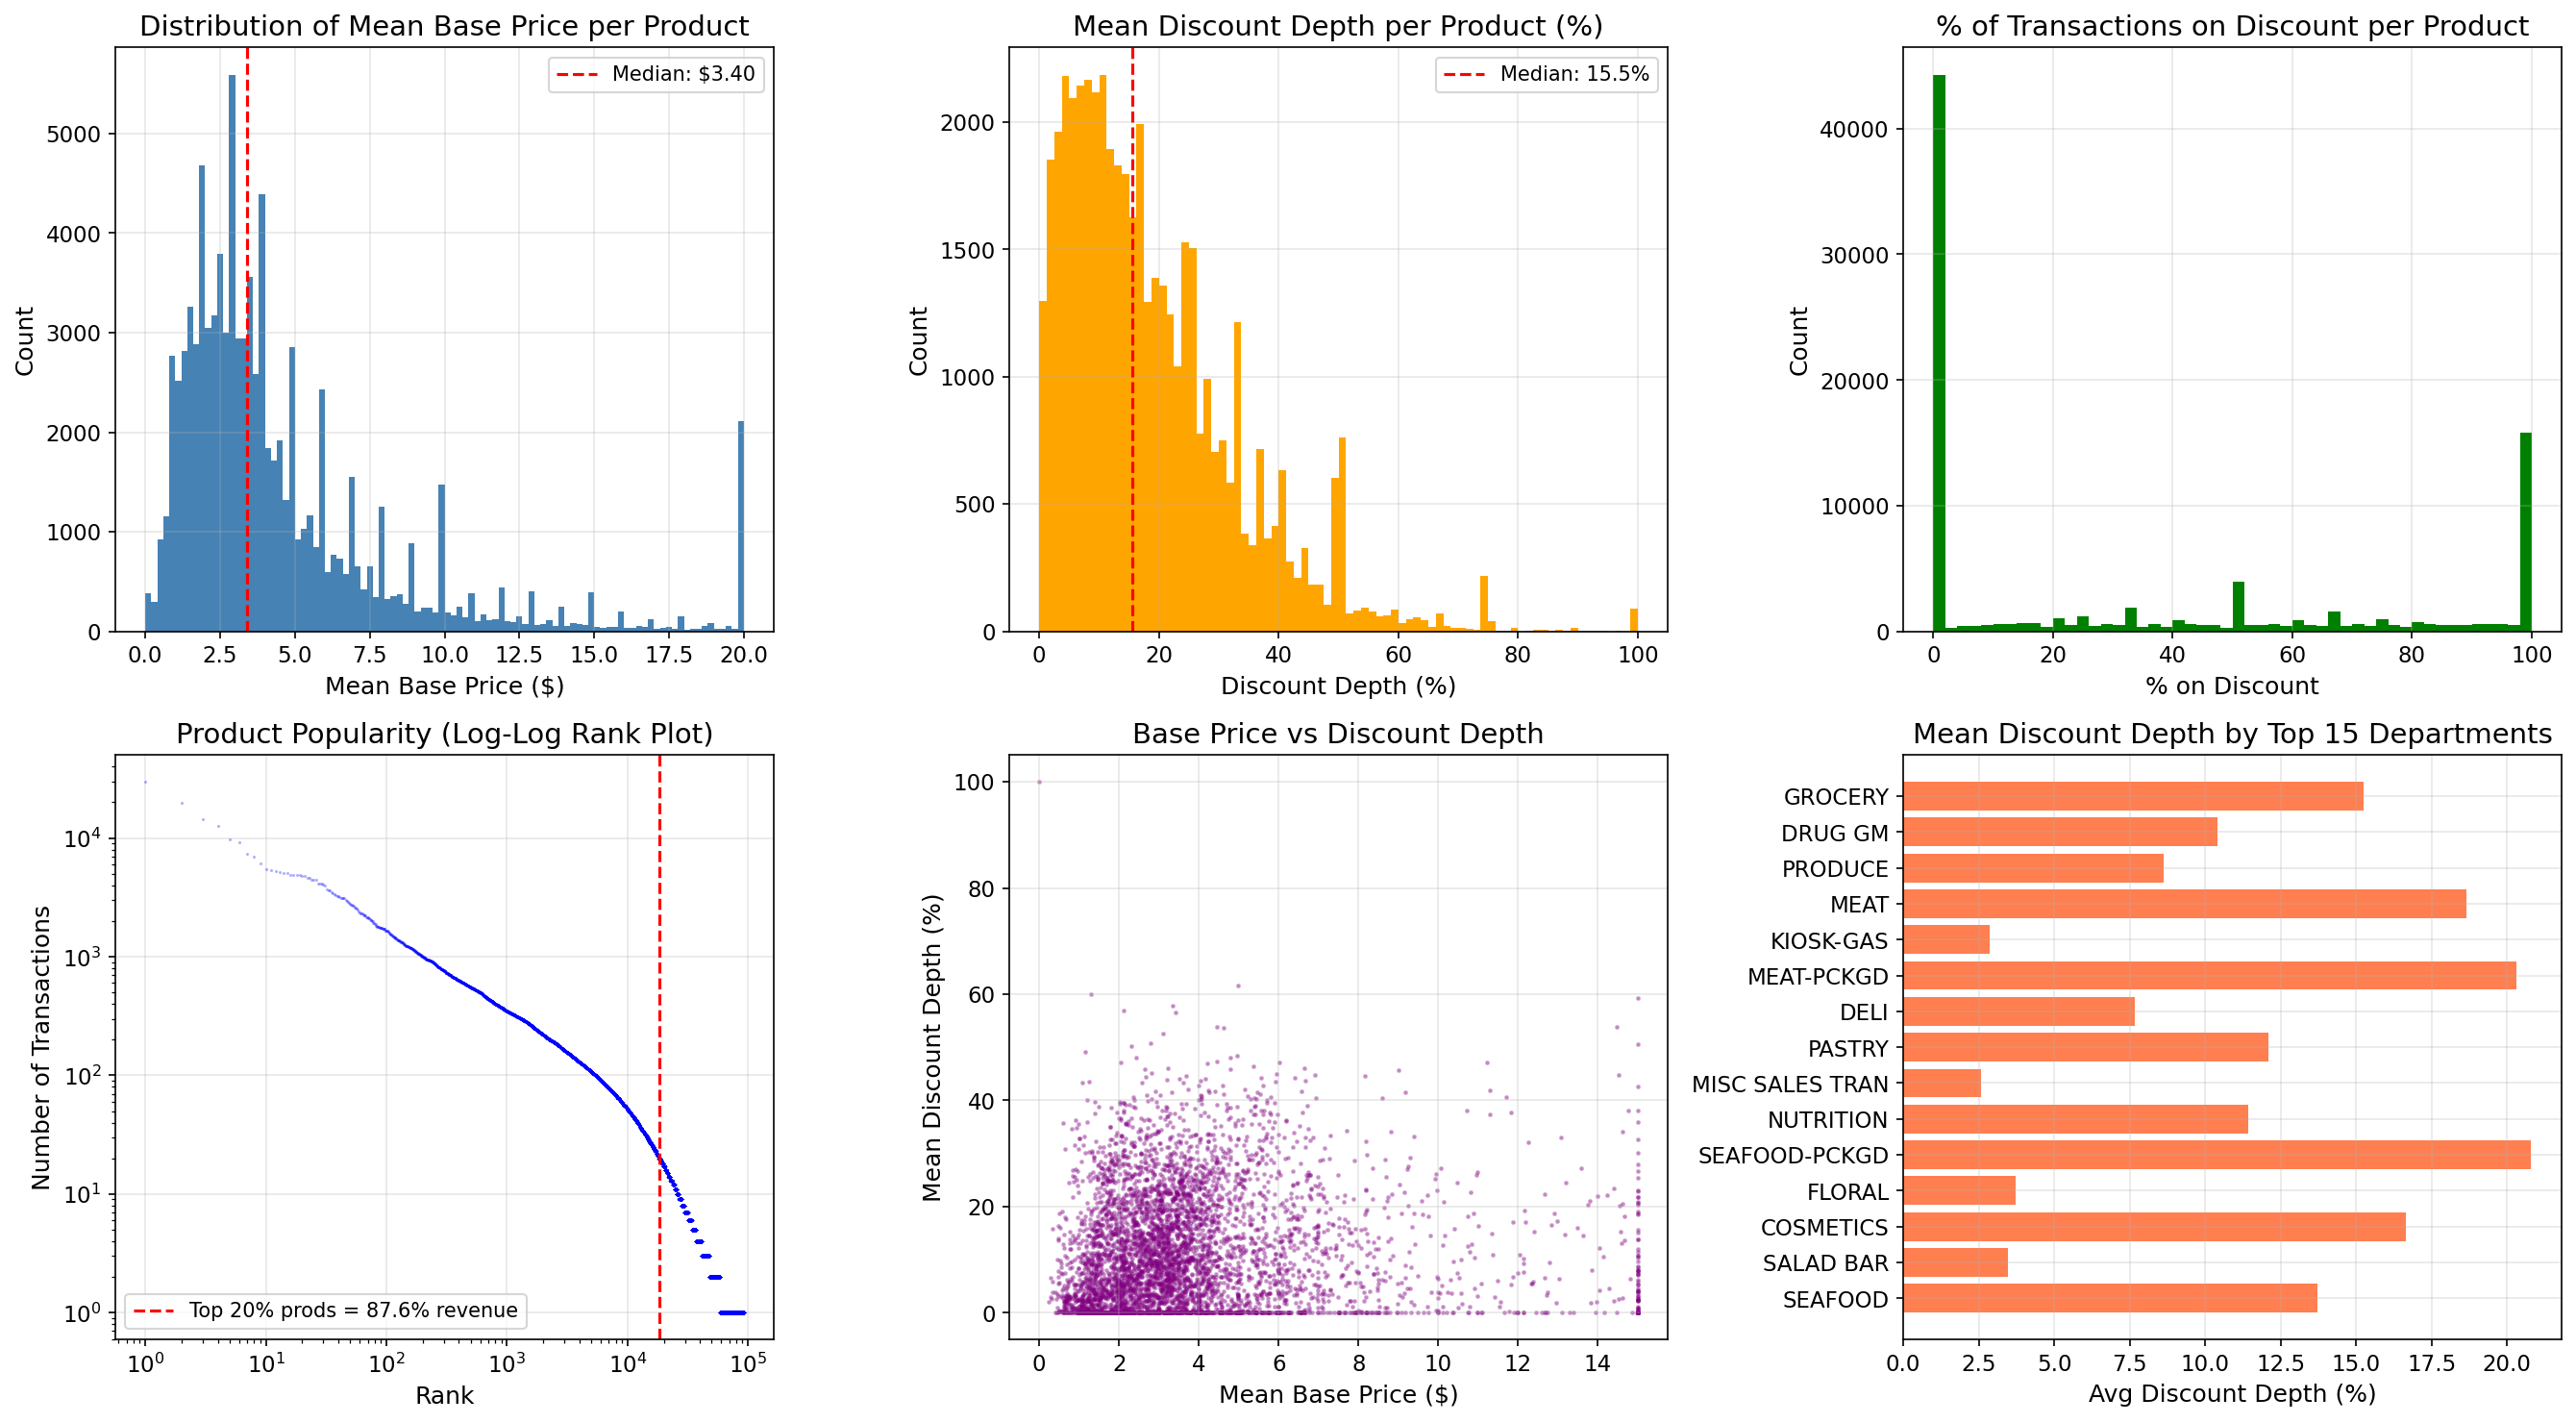
\includegraphics[width=\textwidth]{figures/02_price_discount_patterns.png}
\caption{Distribution of discount depths and their relationship with
unit prices across product categories.}
\label{fig:price-discount}
\end{figure}

\paragraph{Revenue Concentration.}
The revenue distribution across products exhibits extreme Pareto
concentration: the top 0.1\% of products ($\approx$90 SKUs) drive
20\% of total revenue, and the top 1\% account for $\approx$50\%.
This extreme skewness motivates our representative product selection
strategy: rather than attempting to model all 92,339 products, we
select 150 products via stratified revenue-tercile sampling within
segments, drawing 50\% from the top revenue third, 30\% from the
middle third, and 20\% from the bottom third. This ensures the
selected products span the full revenue distribution---covering
high-velocity, mid-range, and long-tail products where promotional
response may differ.

\paragraph{Promotional Exposure.}
Integration of the causal data reveals that 44.9\% of product-week
observations in our estimation panel involve in-store display
exposure (any nonzero display fraction), while 6.7\% involve
mailer/feature advertising. Display exposure is concentrated among
high-velocity products: the Pearson correlation between weekly sales
volume and display probability is $r = 0.31$. This positive
correlation means that omitting display from the demand model would
inflate the discount effect estimate (since discounted products are
often simultaneously displayed).

\begin{figure}[H]
\centering
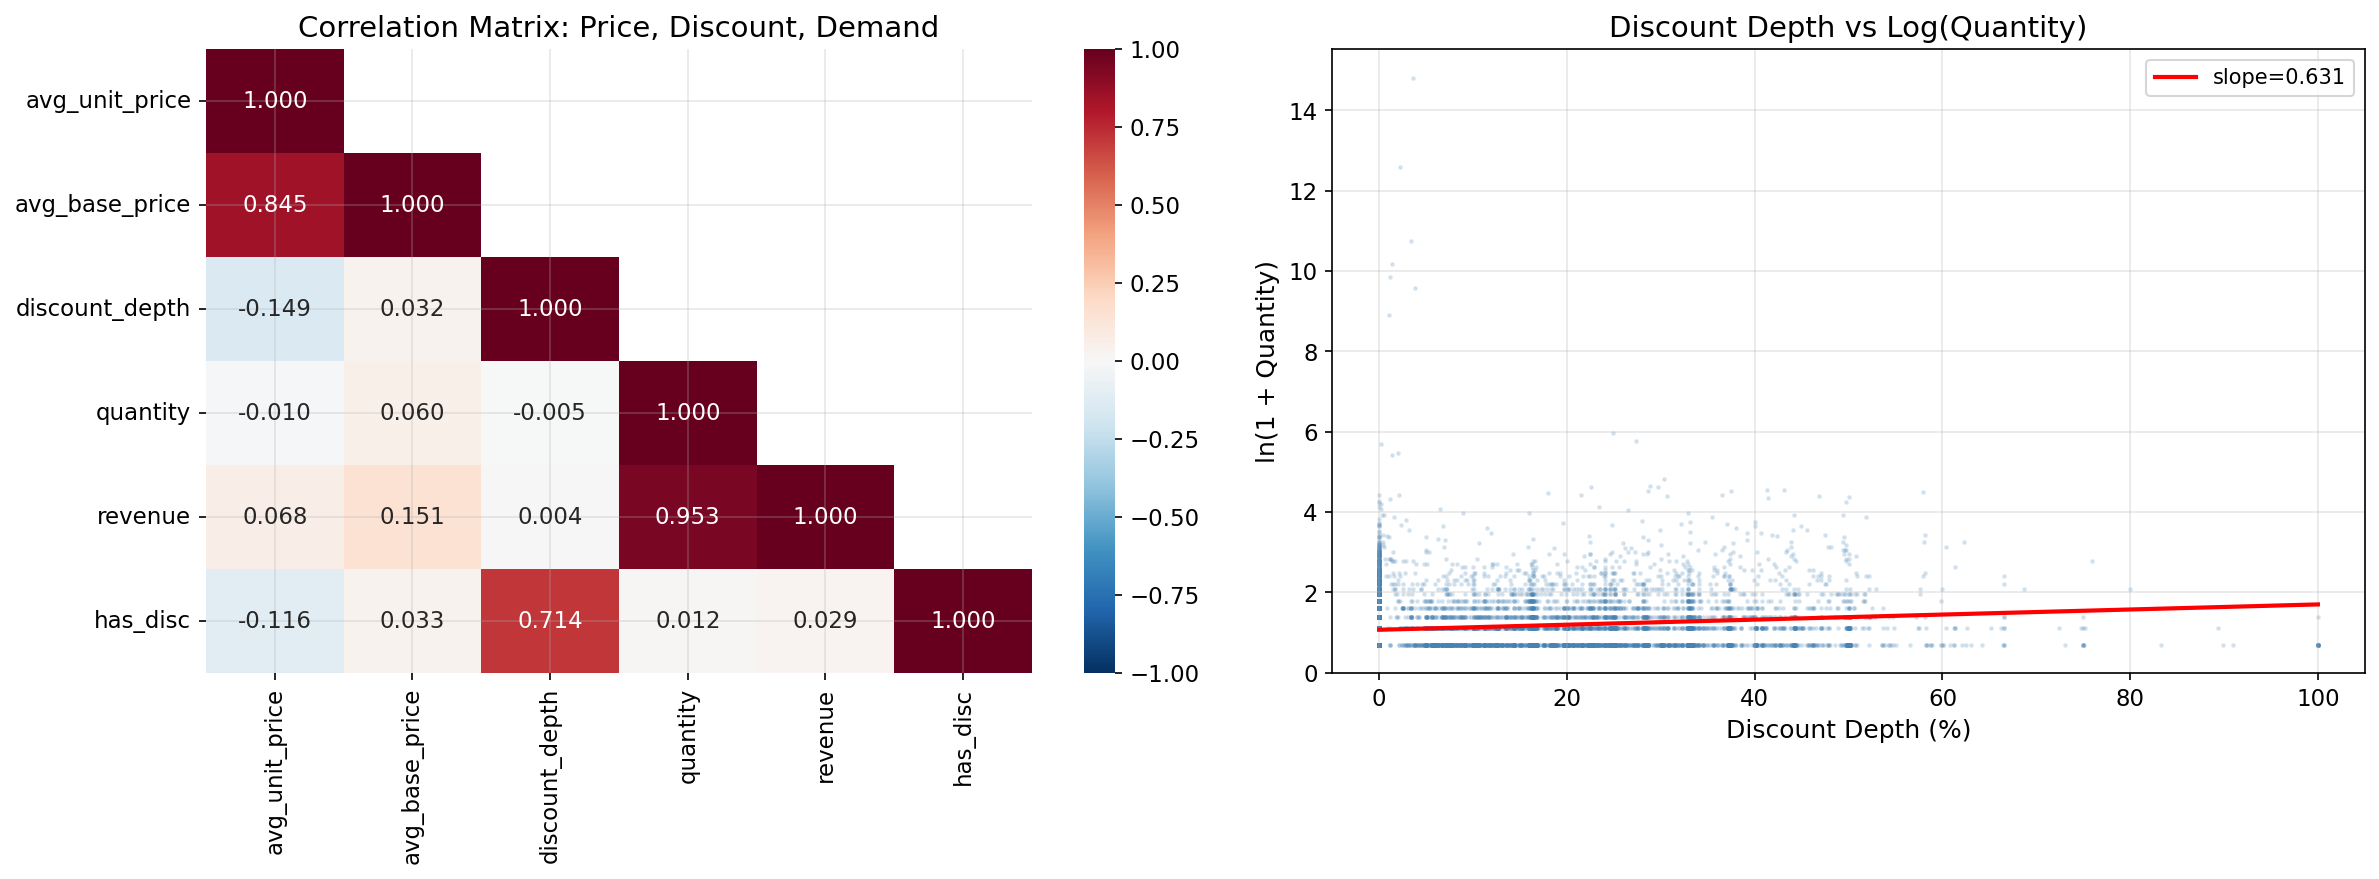
\includegraphics[width=0.85\textwidth]{figures/06_correlation_analysis.png}
\caption{Correlation structure among price, discount, and demand
variables at the product-week level. Note the positive correlation
between display and demand, which must be controlled for in demand
estimation.}
\label{fig:correlation}
\end{figure}

\subsection{Data Quality Review}
\label{sec:data-quality}

Before constructing the estimation panel, we performed a systematic
data quality audit. The key issues identified and their resolutions
are:

\begin{enumerate}[nosep]
\item \textbf{Product returns.} 14,466 transactions (0.56\%) have
$\text{QUANTITY} \leq 0$, representing product returns. These are
removed because a return is not a demand observation and would
produce negative quantities that break the log transform.

\item \textbf{Negative/zero sales.} 18,850 transactions have
$\text{SALES\_VALUE} \leq 0$. These include loss-leader or
heavily-couponed items where net revenue is zero or negative.
Removing them ensures the derived shelf price is strictly positive.

\item \textbf{Zero base prices.} Some transactions produce a
computed base price of zero (e.g., when the discount exactly equals
the gross amount). These are removed as they would produce
$\log(0)$ in the regression.

\item \textbf{Extreme volume outliers.} One product (ID 6534178)
had a median weekly quantity of $\sim$2.9 million units at
\$0.003/unit---likely a weight-based or bulk product measured in
sub-units. We cap the product median log-quantity at the 99.5th
percentile across all products, removing such extreme outliers
from the panel.

\item \textbf{Zero-quantity observations.} After aggregation, 656
product-weeks had exactly zero quantity. These are removed to
preserve the log-linear model's domain.

\item \textbf{Feature period alignment.} Product-level summary
features (mean price, velocity, discount frequency) were initially
computed from all 102 weeks. We restricted this computation to the
stable period (weeks 18--102) to match the panel, preventing
non-stationary ramp-up behavior from distorting the feature space.

\item \textbf{Noisy clustering feature.} The bivariate elasticity
(regressing $\log q$ on $\log p$ without controls) was 57\%
near-zero across products and acted as a noise feature in the
K-Means clustering. Removing it from the five-feature segmentation
improved silhouette scores and eliminated a source of omitted-variable
bias in the segmentation space. The product-level OLS model with
full controls estimates proper elasticities.
\end{enumerate}

After all cleaning filters, 2,576,815 of 2,595,732 raw transactions
(99.3\%) remain.

\subsection{Product-Week Panel Construction}
\label{sec:panel-construction}

The raw transaction data is at household--product--day granularity.
We aggregate to a \textbf{product-week panel}---the fundamental unit
of analysis for demand estimation. The construction proceeds in six
steps:

\begin{enumerate}
\item \textbf{Price and discount derivation.} For each transaction,
compute the shelf price and discount depth using
Eqs.~\eqref{eq:total-discount}--\eqref{eq:discount-depth},
including all three discount components (retail, coupon, and
coupon-match).
Prior to this, we apply data quality filters: remove transactions
with $\text{QUANTITY} \leq 0$ (returns, 14,466 records),
$\text{SALES\_VALUE} \leq 0$ (18,850 records), and
$\text{base\_price} \leq 0$ (zero or negative shelf price,
resulting in 2,576,815 clean transactions from the original
2,595,732).

\item \textbf{Temporal filtering.} Restrict to the stable period
(weeks 18--102), discarding the first 17 weeks which show non-stationary
ramp-up behavior.

\item \textbf{Product-week aggregation.} For each product $i$ and
week $t$, compute:
\begin{itemize}[nosep]
\item $Q_{it}$: total quantity sold (sum across all transactions for
product $i$ in week $t$)
\item $\bar{p}_{it}$: quantity-weighted average shelf price
(total base value divided by total quantity, rather than a simple
mean of transaction unit prices, ensuring the weekly price regressor
reflects the effective price at which units were sold)
\item $\bar{d}_{it}$: mean discount depth
\item $n_{it}$: number of distinct transactions
\end{itemize}

\item \textbf{Causal data merge.} For each product-week, merge in
the continuous display and mailer fractions from the aggregated causal
data (Section~2.3). Product-weeks without causal data are assigned
zero promotional exposure.

\item \textbf{Coupon merge.} Flag product-weeks where the product
has any coupon association.

\item \textbf{Quality filtering.} Retain only products satisfying:
\begin{itemize}[nosep]
\item $\geq 30$ weeks of observations (sufficient temporal coverage
for regression)
\item Coefficient of variation in shelf price $\geq 0.03$ (sufficient
price variation for elasticity identification)
\item No zero-quantity observations (removed after aggregation)
\item Median log-quantity below the 99.5th percentile across all
products (removes extreme volume outliers such as bulk/weight items)
\end{itemize}
\end{enumerate}

The resulting panel contains \textbf{343,375 product-week
observations} across \textbf{6,443 eligible products}.
Table~\ref{tab:panel-stats} summarizes the key panel statistics.

\begin{table}[H]
\centering
\caption{Product-week panel descriptive statistics.}
\label{tab:panel-stats}
\begin{tabular}{l rrrr}
\toprule
\textbf{Variable} & \textbf{Mean} & \textbf{Median} &
\textbf{P5} & \textbf{P95} \\
\midrule
Quantity ($Q_{it}$) & 22.3 & 7 & 1 & 78 \\
Shelf price (\$) & 4.87 & 3.49 & 0.99 & 13.99 \\
Discount depth (\%) & 8.1 & 0 & 0 & 38.2 \\
Display fraction & 0.449 & 0 & 0 & 1 \\
Mailer fraction & 0.067 & 0 & 0 & 0 \\
Weeks per product & 54.6 & 56 & 31 & 78 \\
\bottomrule
\end{tabular}
\end{table}

%% ═══════════════════════════════════════════════════════════
\section{Product Segmentation}
\label{sec:segmentation}
%% ═══════════════════════════════════════════════════════════

\subsection{Segmentation Features}

We segment products using K-Means clustering on five standardized
features:

\begin{enumerate}[nosep]
\item \textbf{Log price}: $\log(\bar{p}_i)$, the mean shelf price
\item \textbf{Log velocity}: $\log(\bar{q}_i / T)$, weekly sales rate
\item \textbf{Discount frequency}: fraction of weeks with
$d_{it} > 0$
\item \textbf{Mean discount depth}: average $d_{it}$ when discounted
\item \textbf{Price coefficient of variation}: $\text{CV}(p_{it})$
\end{enumerate}

Earlier iterations of the segmentation included a sixth feature---a
preliminary bivariate log-log elasticity. Critical review revealed
that 57\% of products had near-zero bivariate elasticity (due to
limited shelf-price variation), making this feature dominated by
noise. Dropping it improved silhouette scores and removed a source
of omitted-variable bias in the segmentation space.

\subsection{Cluster Selection}

We evaluate $K \in \{5, 6, \ldots, 25\}$ using silhouette scores
and inertia (within-cluster sum of squares). We select $K = 12$
based on the elbow in inertia and acceptable silhouette scores.

\begin{figure}[H]
\centering
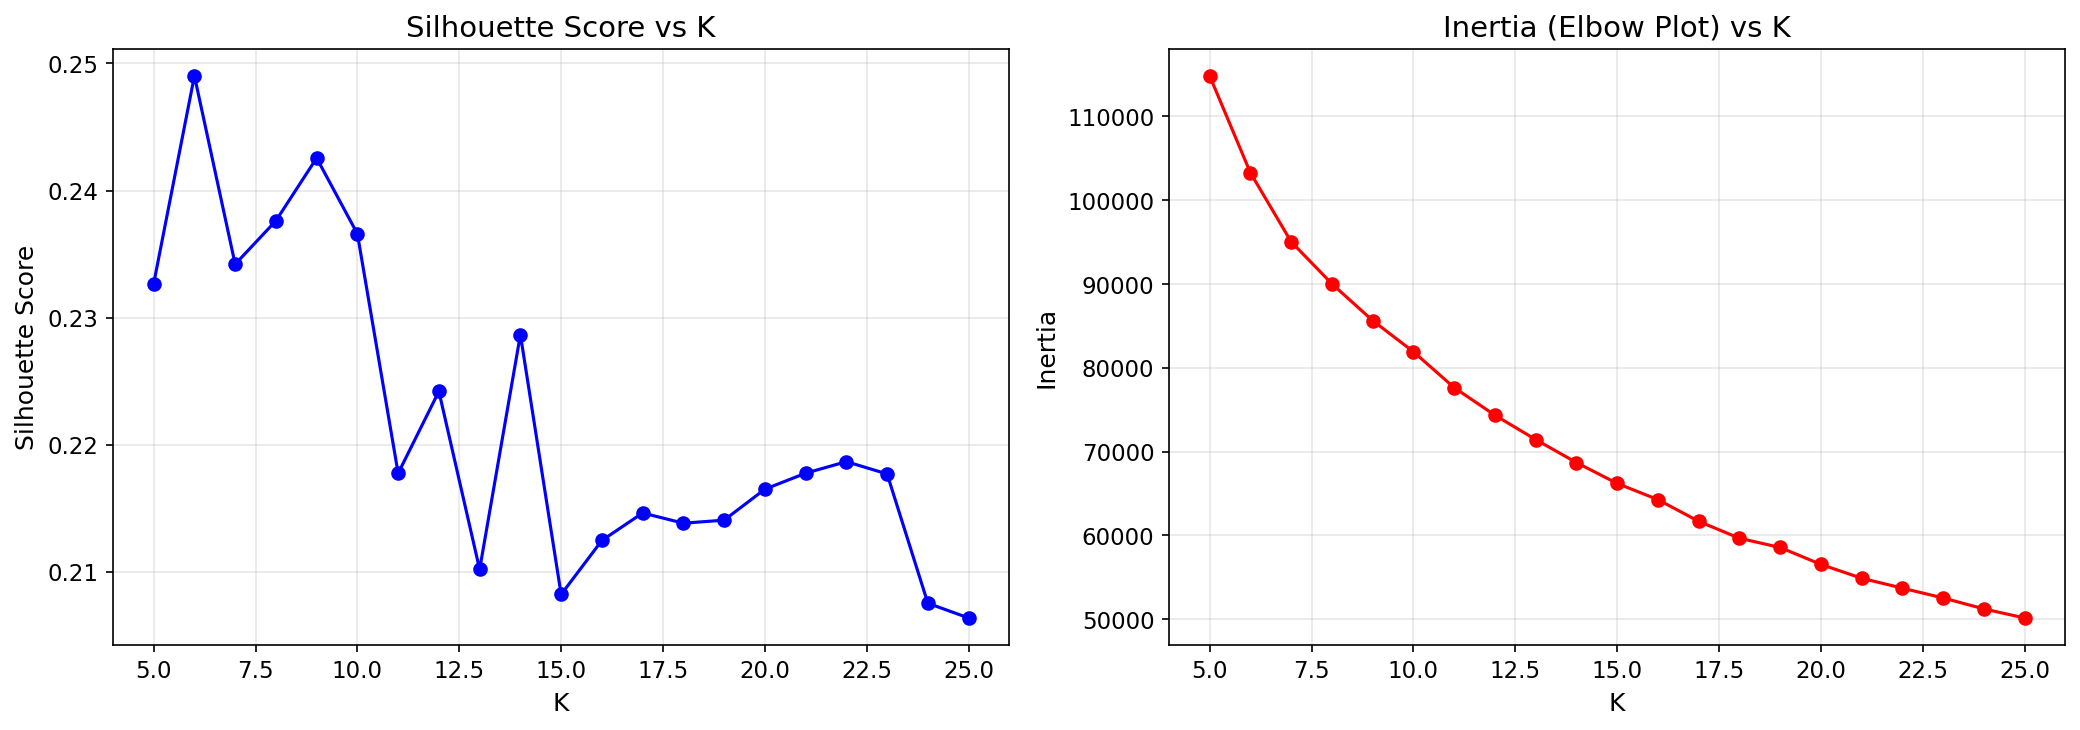
\includegraphics[width=0.85\textwidth]{figures/07_kmeans_evaluation.png}
\caption{K-Means evaluation: inertia (left) and silhouette score
(right) across $K = 5$--$25$. $K = 12$ balances parsimony with
within-cluster homogeneity.}
\label{fig:kmeans-eval}
\end{figure}

\subsection{Representative Product Selection}

From the 6,443 eligible products segmented into 12 clusters, we
select 150 representative products using \textbf{stratified
revenue-tercile sampling} within each segment. Products in each
segment are divided into three revenue tiers (top, middle, and
bottom thirds), and representatives are drawn proportionally:
50\% from the top tier, 30\% from the middle tier, and 20\% from
the bottom tier. This stratification ensures the selected products
span the full revenue distribution within each segment, avoiding
head-SKU bias that would over-represent high-velocity items and
under-represent long-tail products where promotional response may
differ. Each representative product must have
$\geq 30$ weeks of data and price CV $\geq 0.03$,
with a minimum allocation of 2 products per segment to avoid
singleton segments that would make shrinkage degenerate.

Of the 12 clusters, 11 are represented in the final 150-product
selection; one segment (Segment~3) has no products allocated due to
its low revenue share relative to the allocation algorithm's
rounding. All 150 selected products are successfully fitted.

Table~\ref{tab:seg-allocation} shows the segment allocation and
post-shrinkage demand characteristics.

\begin{table}[H]
\centering
\caption{Segment allocation of 150 representative products with
post-shrinkage parameter summaries. Elasticities shown after
shrinkage and non-positivity constraint.}
\label{tab:seg-allocation}
\begin{tabular}{crrrr}
\toprule
\textbf{Seg.} & \textbf{Products} & \textbf{Med.\ Elast.} &
\textbf{Med.\ Disc Eff.} & \textbf{Mean Price (\$)} \\
\midrule
0 & 7 & $-0.140$ & 2.34 & 4.46 \\
1 & 2 & $-0.244$ & 0.87 & 4.10 \\
2 & 3 & $0.000$ & 2.32 & 10.27 \\
4 & 31 & $-1.067$ & 1.24 & 3.59 \\
5 & 15 & $-0.309$ & 1.55 & 1.59 \\
6 & 44 & $-0.173$ & 3.18 & 5.79 \\
7 & 6 & $0.000$ & 0.07 & 13.34 \\
8 & 7 & $-1.241$ & 2.90 & 13.65 \\
9 & 29 & $-0.430$ & 0.89 & 4.85 \\
10 & 2 & $0.000$ & $-2.69$ & 1.01 \\
11 & 4 & $0.000$ & $0.00$ & 18.77 \\
\midrule
\textbf{Total} & \textbf{150} & $-0.215$ & 1.98 & --- \\
\bottomrule
\end{tabular}
\end{table}

\noindent All 150 products have non-positive elasticity after
shrinkage and the enforcement of the economic sign constraint
($\hat{\varepsilon}_i \leq 0$). Products showing zero median
elasticity in the table have OLS estimates that were either positive
(and thus clipped to zero) or near zero before shrinkage.

\begin{figure}[H]
\centering
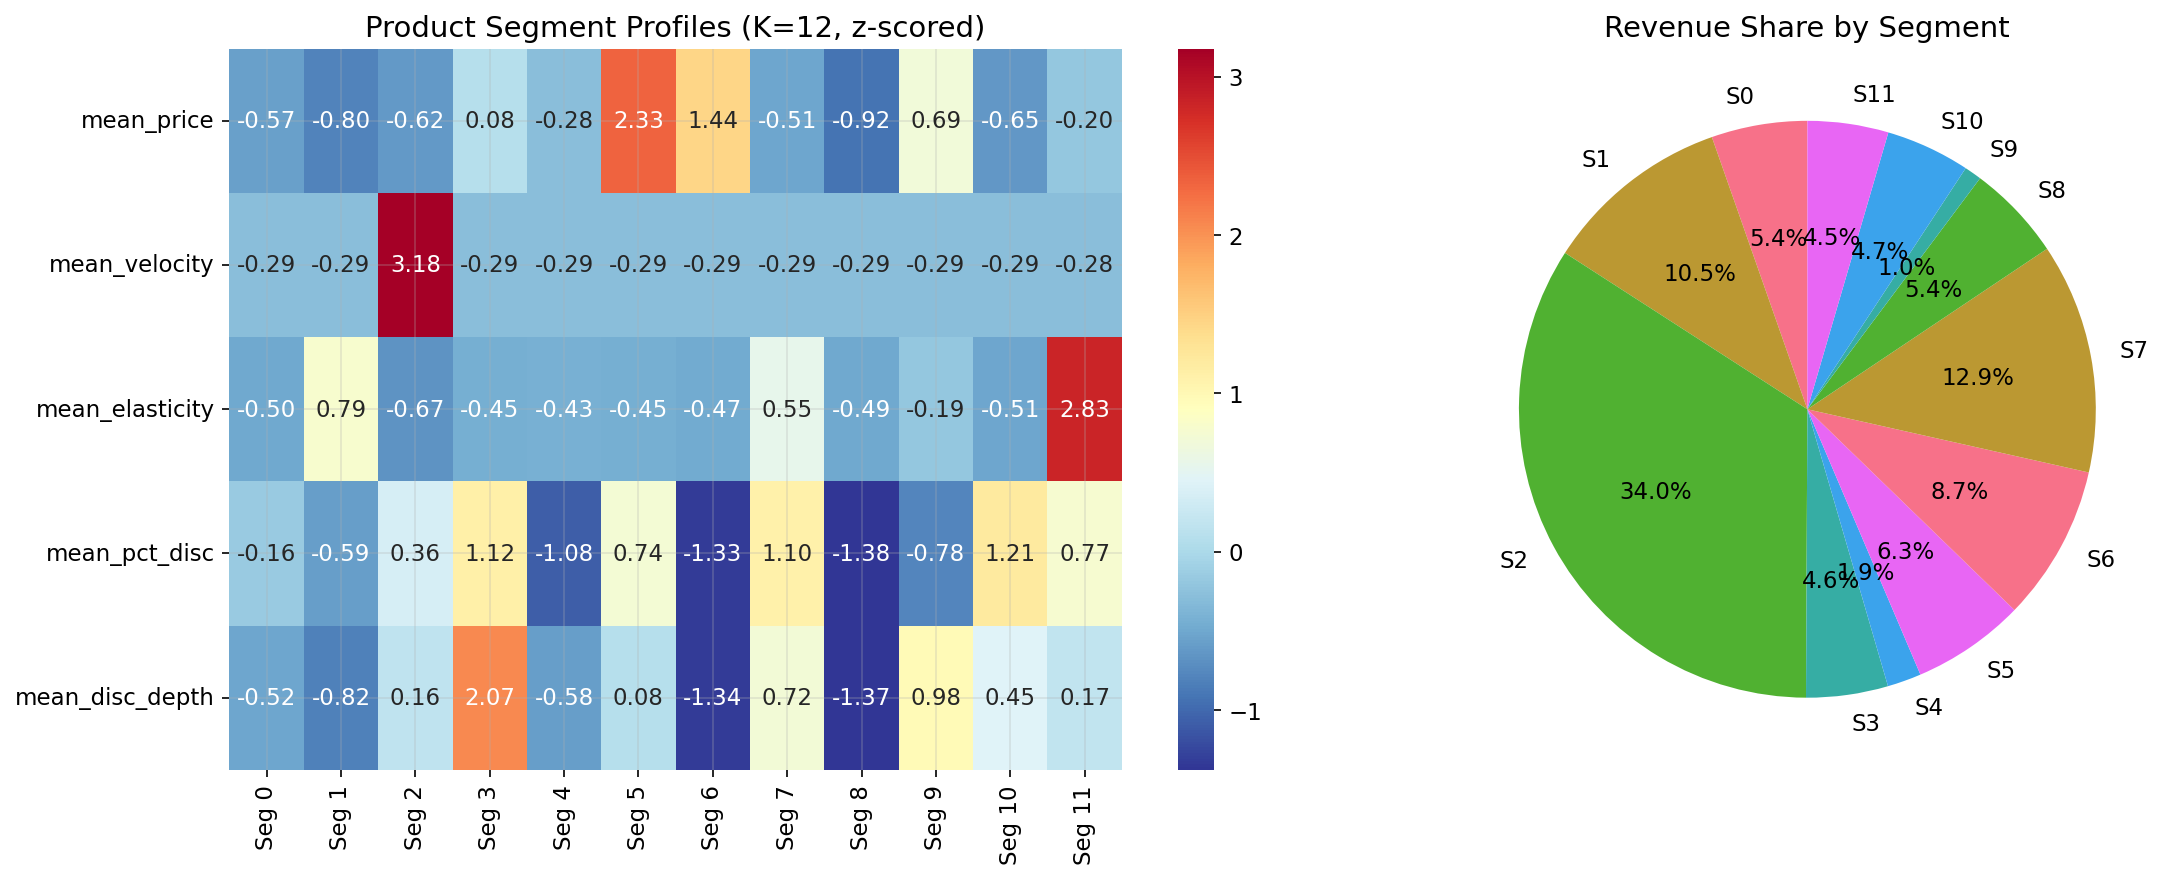
\includegraphics[width=\textwidth]{figures/08_product_segments.png}
\caption{Product segments in the log-price vs.\ log-velocity space,
colored by cluster assignment.}
\label{fig:product-segments}
\end{figure}

%% ═══════════════════════════════════════════════════════════
\section{Demand Model Estimation}
\label{sec:demand}
%% ═══════════════════════════════════════════════════════════

\subsection{Model Specification}

We estimate demand models at the \textbf{individual product level}.
For each product $i$ with sufficient temporal coverage, we fit a
separate model using product-week panel data.

\subsubsection{Log-Log OLS with Promotional Controls (Baseline)}

The primary model is a log-linear demand specification with AR(1)
demand persistence and within-segment cross-product substitution:

\begin{equation}
\label{eq:loglog}
\begin{aligned}
\ln Q_{it} &= \alpha_i + \varepsilon_i \ln p_{it}^{\text{shelf}}
+ \gamma_i \, d_{it}
+ \rho_i \, \ln Q_{i,t-1} \\
&\quad + \lambda_i \, \overline{d}_{-i,s(i),t}
+ \delta_i^D \, \text{display\_pct}_{it}
+ \delta_i^M \, \text{mailer\_pct}_{it} \\
&\quad + \beta_{i,1} \cos\!\left(\frac{2\pi w_t}{52}\right)
+ \beta_{i,2} \sin\!\left(\frac{2\pi w_t}{52}\right)
+ u_{it}
\end{aligned}
\end{equation}

where:
\begin{itemize}[nosep]
\item $Q_{it}$: total quantity sold of product $i$ in week $t$
\item $p_{it}^{\text{shelf}}$: quantity-weighted average shelf
(pre-discount) price per unit
\item $d_{it} \in [0, 1]$: continuous discount depth (fraction of
shelf price discounted)
\item $\ln Q_{i,t-1}$: lagged log-demand, capturing AR(1)
persistence in the demand process. The coefficient $\rho_i$
measures how much of the previous period's demand carries forward.
A positive $\rho_i$ means demand is ``sticky''---a good (bad) week
tends to be followed by another good (bad) week
\item $\overline{d}_{-i,s(i),t}$: the mean discount depth of
\emph{other} products in the same segment $s(i)$ in week $t$.
The coefficient $\lambda_i$ captures cross-product substitution:
a negative $\lambda_i$ means competitors' discounts cannibalize
own demand
\item $\text{display\_pct}_{it} \in [0,1]$: fraction of stores with
in-store display exposure (continuous, from causal data)
\item $\text{mailer\_pct}_{it} \in [0,1]$: fraction of stores with
mailer/feature advertising exposure (continuous)
\item $w_t$: week number (for annual seasonality via Fourier terms)
\item $u_{it}$: error term
\end{itemize}

Equation~\eqref{eq:loglog} uses heteroskedasticity-consistent
standard errors (HC1) for robust inference. Observations are sorted
chronologically and the first observation per product is dropped
(no lag available), requiring a minimum of 10 valid observations.
The lagged demand term $\ln Q_{i,t-1}$ makes the demand process
genuinely \emph{dynamic}: the simulator's state variable $q_t$ now
\emph{causally} influences the demand transition, not just
observationally. The cross-product substitution term
$\overline{d}_{-i,s(i),t}$ makes products \emph{interdependent}:
the discount decision for one product affects demand for others in
the same segment.

We note that $\varepsilon_i$ captures the elasticity of demand with
respect to the \emph{shelf price} (holding discount depth constant),
while $\gamma_i$ captures the \emph{promotional effect} of discount
depth (holding shelf price constant). The display and mailer
covariates enter as continuous fractions, preserving the intensity of
promotional exposure rather than collapsing it to binary incidence.

\subsubsection{Machine Learning Benchmarks}

We compare the log-log OLS against four ML alternatives, all fitted
at the per-product level:

\begin{itemize}[nosep]
\item \textbf{Random Forest} (100 trees, max depth 8): nonparametric
flexible model; features: $\log p$, $d$, display\_pct, mailer\_pct.
\item \textbf{XGBoost} (100 rounds, max depth 5, lr 0.1): gradient
boosted trees with continuous promotional features.
\item \textbf{LightGBM} (same hyperparameters): histogram-based
gradient boosting.
\item \textbf{Neural Network} (32-16 hidden units, 200 epochs):
feedforward network with ReLU activations and dropout.
\end{itemize}

For tree-based and neural models, we extract summary parameters
(elasticity and discount effect) via finite-difference
approximation evaluated at the training data centroid. These
summary parameters enable integration with the log-linear simulator,
but we note that this two-parameter compression is not equivalent to
simulating the original ML model---it is a necessary structural
approximation for simulator compatibility (see
Section~\ref{sec:discussion}).

\subsection{Empirical Bayes Shrinkage}
\label{sec:shrinkage}

With only 61 observations per product (median), individual
parameter estimates can be noisy. We regularize using James--Stein
empirical Bayes shrinkage toward segment medians:

\begin{equation}
\hat{\theta}_i^{\text{shrunk}} = w_i \hat{\theta}_i^{\text{OLS}}
+ (1 - w_i) \, \tilde{\theta}_{s(i)}
\end{equation}

where $\tilde{\theta}_{s(i)}$ is the median of segment $s(i)$
containing product $i$, and:

\begin{equation}
\label{eq:js-weight}
w_i = \frac{\hat{\sigma}_{s}^2}
{\hat{\sigma}_{s}^2 + \hat{\sigma}_{\theta,i}^2}
\end{equation}

Here $\hat{\sigma}_{s}^2$ is the across-product variance of
$\hat{\theta}$ within the segment and $\hat{\sigma}_{\theta,i}^2$
is the parameter-specific estimation variance for product $i$.

\paragraph{Parameter-specific standard errors.}
For the elasticity and discount effect parameters, we use the HC1
standard errors from the OLS regression ($\text{SE}(\hat{\varepsilon}_i)$
and $\text{SE}(\hat{\gamma}_i)$) rather than a generic
$\hat{\sigma}_i^2 / n_i$ proxy. This aligns the shrinkage weight with
the actual uncertainty in each coefficient: a product with high price
variation has a precisely estimated elasticity (high $w_i$, less
shrinkage) even if its residual variance is large. For display and
mailer effects, we fall back to $\hat{\sigma}_i^2 / n_i$ as a
variance proxy.

\paragraph{Shrinkage scope.}
Shrinkage is applied to six parameters: (1)~elasticity
$\hat{\varepsilon}_i$, (2)~discount effect $\hat{\gamma}_i$,
(3)~demand persistence $\hat{\rho}_i$,
(4)~substitution effect $\hat{\lambda}_i$,
(5)~display effect $\hat{\delta}_i^D$, and (6)~mailer effect
$\hat{\delta}_i^M$, each toward their respective segment medians.
The shrinkage weight is capped at 0.9 to prevent any single estimate
from being fully trusted.

\paragraph{Handling degenerate segments.}
To prevent degenerate shrinkage from singleton segments, the
representative selector enforces a minimum of 2 products per
segment. For any segment where the within-segment
variance $\hat{\sigma}_s^2$ is undefined or near-zero, we fall
back to the \emph{global} across-product variance computed over all
150 products, ensuring a finite shrinkage weight.

\paragraph{Post-shrinkage winsorization and sign constraints.}
After shrinkage, all shrunk parameters are winsorized at the 2.5th
and 97.5th percentiles to prevent extreme values from dominating the
simulator. Then three economic sign constraints are imposed:
(i)~elasticities are clipped to non-positive
($\hat{\varepsilon}_i^{\text{shrunk}} \leq 0$) to enforce the
law of demand; (ii)~demand persistence is clipped to $[0, 0.95]$
to enforce stationarity and the economic expectation that demand
should not negatively persist; (iii)~substitution effects are
clipped to non-positive ($\hat{\lambda}_i^{\text{shrunk}} \leq 0$)
to enforce that competitor discounting can only cannibalize, not
boost, own demand. These are deliberate structural constraints
imposed for simulator stability, not direct outputs of the
estimation.

\subsection{Intercept Calibration}
\label{sec:calibration}

To ensure mean predictions match observed demand levels, we
calibrate the intercept for each product. The calibration absorbs the
mean contributions of all regressors:

\begin{equation}
\label{eq:intercept-cal}
\hat{\alpha}_i^{\text{cal}} = \ln \bar{Q}_i
- \hat{\varepsilon}_i^{\text{shrunk}} \ln \bar{p}_i
- \hat{\gamma}_i^{\text{shrunk}} \bar{d}_i
- \hat{\delta}_{i}^{D,\text{shrunk}} \overline{\text{display}}_i
- \hat{\delta}_{i}^{M,\text{shrunk}} \overline{\text{mailer}}_i
- \hat{\lambda}_{i}^{\text{shrunk}} \overline{d}_{-i,s(i)}
\end{equation}

where $\bar{Q}_i$, $\bar{p}_i$, $\bar{d}_i$,
$\overline{\text{display}}_i$, $\overline{\text{mailer}}_i$, and
$\overline{d}_{-i,s(i)}$ are the \emph{training-set} means of
quantity, shelf price, discount depth, display fraction, mailer
fraction, and within-segment competitor discount depth for product
$i$. The AR(1) persistence term does not require calibration because
the mean deviation of lagged log-demand from its own training mean
is zero by construction.

\paragraph{Why calibrate?}
The raw OLS intercept $\hat{\alpha}_i$ is estimated jointly with all
regressors and its numerical value depends on the units and centering
of the covariates. After applying shrinkage to the slope
coefficients (which changes them from their OLS values), the raw
intercept no longer reproduces the observed mean demand. Including
the mean display and mailer effects in the calibration ensures that
the simulator's baseline demand at average promotional conditions
matches the historically observed sales level.

\subsection{Bias Correction}

Because the model operates in log-space but the simulator requires
level-space demand, we apply the Duan (1983) smearing retransformation
correction:

\begin{equation}
\hat{\phi} = \frac{\sum_i \sum_t Q_{it}}
{\sum_i \sum_t \exp\bigl(\hat{\alpha}_i^{\text{cal}}
+ \hat{\varepsilon}_i^{\text{shrunk}} \ln p_{it}
+ \hat{\gamma}_i^{\text{shrunk}} d_{it}
+ \hat{\rho}_i^{\text{shrunk}} (\ln Q_{i,t-1} - \overline{\ln Q}_i)
+ \hat{\lambda}_i^{\text{shrunk}} (\overline{d}_{-i,s(i),t} - \overline{d}_{-i,s(i)})
+ \hat{\delta}_{i}^{D,\text{shrunk}} \text{display\_pct}_{it}
+ \hat{\delta}_{i}^{M,\text{shrunk}} \text{mailer\_pct}_{it}
\bigr)}
\end{equation}

The Duan correction $\hat{\phi}$ now includes the AR(1) persistence
and substitution terms in the denominator, ensuring the bias factor
accounts for all systematic demand components. For the calibrated
OLS model, $\hat{\phi} = 0.698$, indicating that the raw log-space
predictions over-predict level-space demand by approximately 30\%.
This bias arises from Jensen's inequality ($E[\exp(X)] > \exp(E[X])$)
and is amplified by the additional variance contributed by the
persistence and substitution terms. The Duan correction rescales
all predictions to match aggregate observed demand.

%% ═══════════════════════════════════════════════════════════
\section{Model Comparison}
\label{sec:comparison}
%% ═══════════════════════════════════════════════════════════

\subsection{Evaluation Protocol}

We split the panel temporally: weeks 18--82 for training (7,473
observations across the 150 representative products after dropping
the first observation per product to form the AR(1) lag) and weeks
83--102 for testing (2,359 observations). All metrics are computed
on the test set.

\subsection{Results}

Table~\ref{tab:model-comparison} presents the model comparison
results.

\begin{table}[H]
\centering
\caption{Demand model comparison on test data ($N = 150$ products).
Best value in each column is \textbf{bolded}. All models use
continuous display and mailer fractions as promotional features.
The log-log OLS additionally includes AR(1) persistence and
within-segment substitution.}
\label{tab:model-comparison}
\begin{tabular}{l ccc cc}
\toprule
\textbf{Model} &
\textbf{Mean $R^2$} &
\textbf{Log $r$} &
\textbf{MAPE (\%)} &
\textbf{Lift $r$} &
\textbf{Dir.\ (\%)} \\
\midrule
Log-Log OLS & 0.363 & 0.621 & 46.1 & \textbf{0.694} & 77.8 \\
Random Forest & 0.551 & \textbf{0.715} & \textbf{18.0} & 0.503 & 72.2 \\
XGBoost & \textbf{0.606} & 0.704 & 22.4 & 0.480 & 68.5 \\
LightGBM & 0.156 & 0.694 & 21.2 & 0.171 & 50.9 \\
Neural Network & 0.365 & 0.055 & $\infty$ & $-0.063$ & \textbf{71.7} \\
\bottomrule
\end{tabular}
\end{table}

\paragraph{Key Findings.}

\begin{enumerate}[nosep]
\item \textbf{OLS selected for structural compatibility.} The
simulator requires structurally interpretable elasticity, discount
effect, persistence, and substitution parameters. While Random
Forest achieves higher log correlation (0.715 vs.\ 0.621), the ML
models' finite-difference elasticities are not direct structural
parameters---they are local approximations that may not generalize
when the simulator applies them globally over discount sweeps. OLS
is preferred because its parameters directly enter the simulator's
demand equation, and its lift correlation (0.694) is the strongest
among all models.

\item \textbf{OLS achieves the strongest lift correlation (0.694).}
The lift correlation measures how well the model ranks products by
their demand response to discounting---the most critical metric for
the simulator, which relies on
$\hat{\gamma}_i^{\text{shrunk}}$ to generate revenue differences
across discount policies. OLS substantially outperforms all ML
models on this metric.

\item \textbf{OLS MAPE is higher than before (46.1\%).} The
inclusion of AR(1) lagged demand and cross-product substitution as
regressors adds model complexity. The first observation per product
is dropped (no lag), reducing the effective training sample. The
MAPE increase reflects the tradeoff between capturing richer market
dynamics and out-of-sample prediction accuracy. Despite the higher
MAPE, the OLS model retains its superior lift correlation, which is
the metric most relevant for the simulator's policy evaluation.

\item \textbf{Tree models overfit less with stratified sampling.}
With stratified representative selection, the tree models now
achieve more moderate in-sample R$^2$ values (0.551 for RF, 0.606
for XGBoost) and better out-of-sample MAPEs (18.0\% and 22.4\%)
compared to prior runs, suggesting the stratified sample is harder
to overfit.

\item \textbf{Neural network remains unstable.} With only
$\sim$49 training observations per product (after lag-dropping),
the 32-16 feedforward network is overparameterized and produces
divergent MAPE and negative lift correlation.
\end{enumerate}

\begin{figure}[H]
\centering
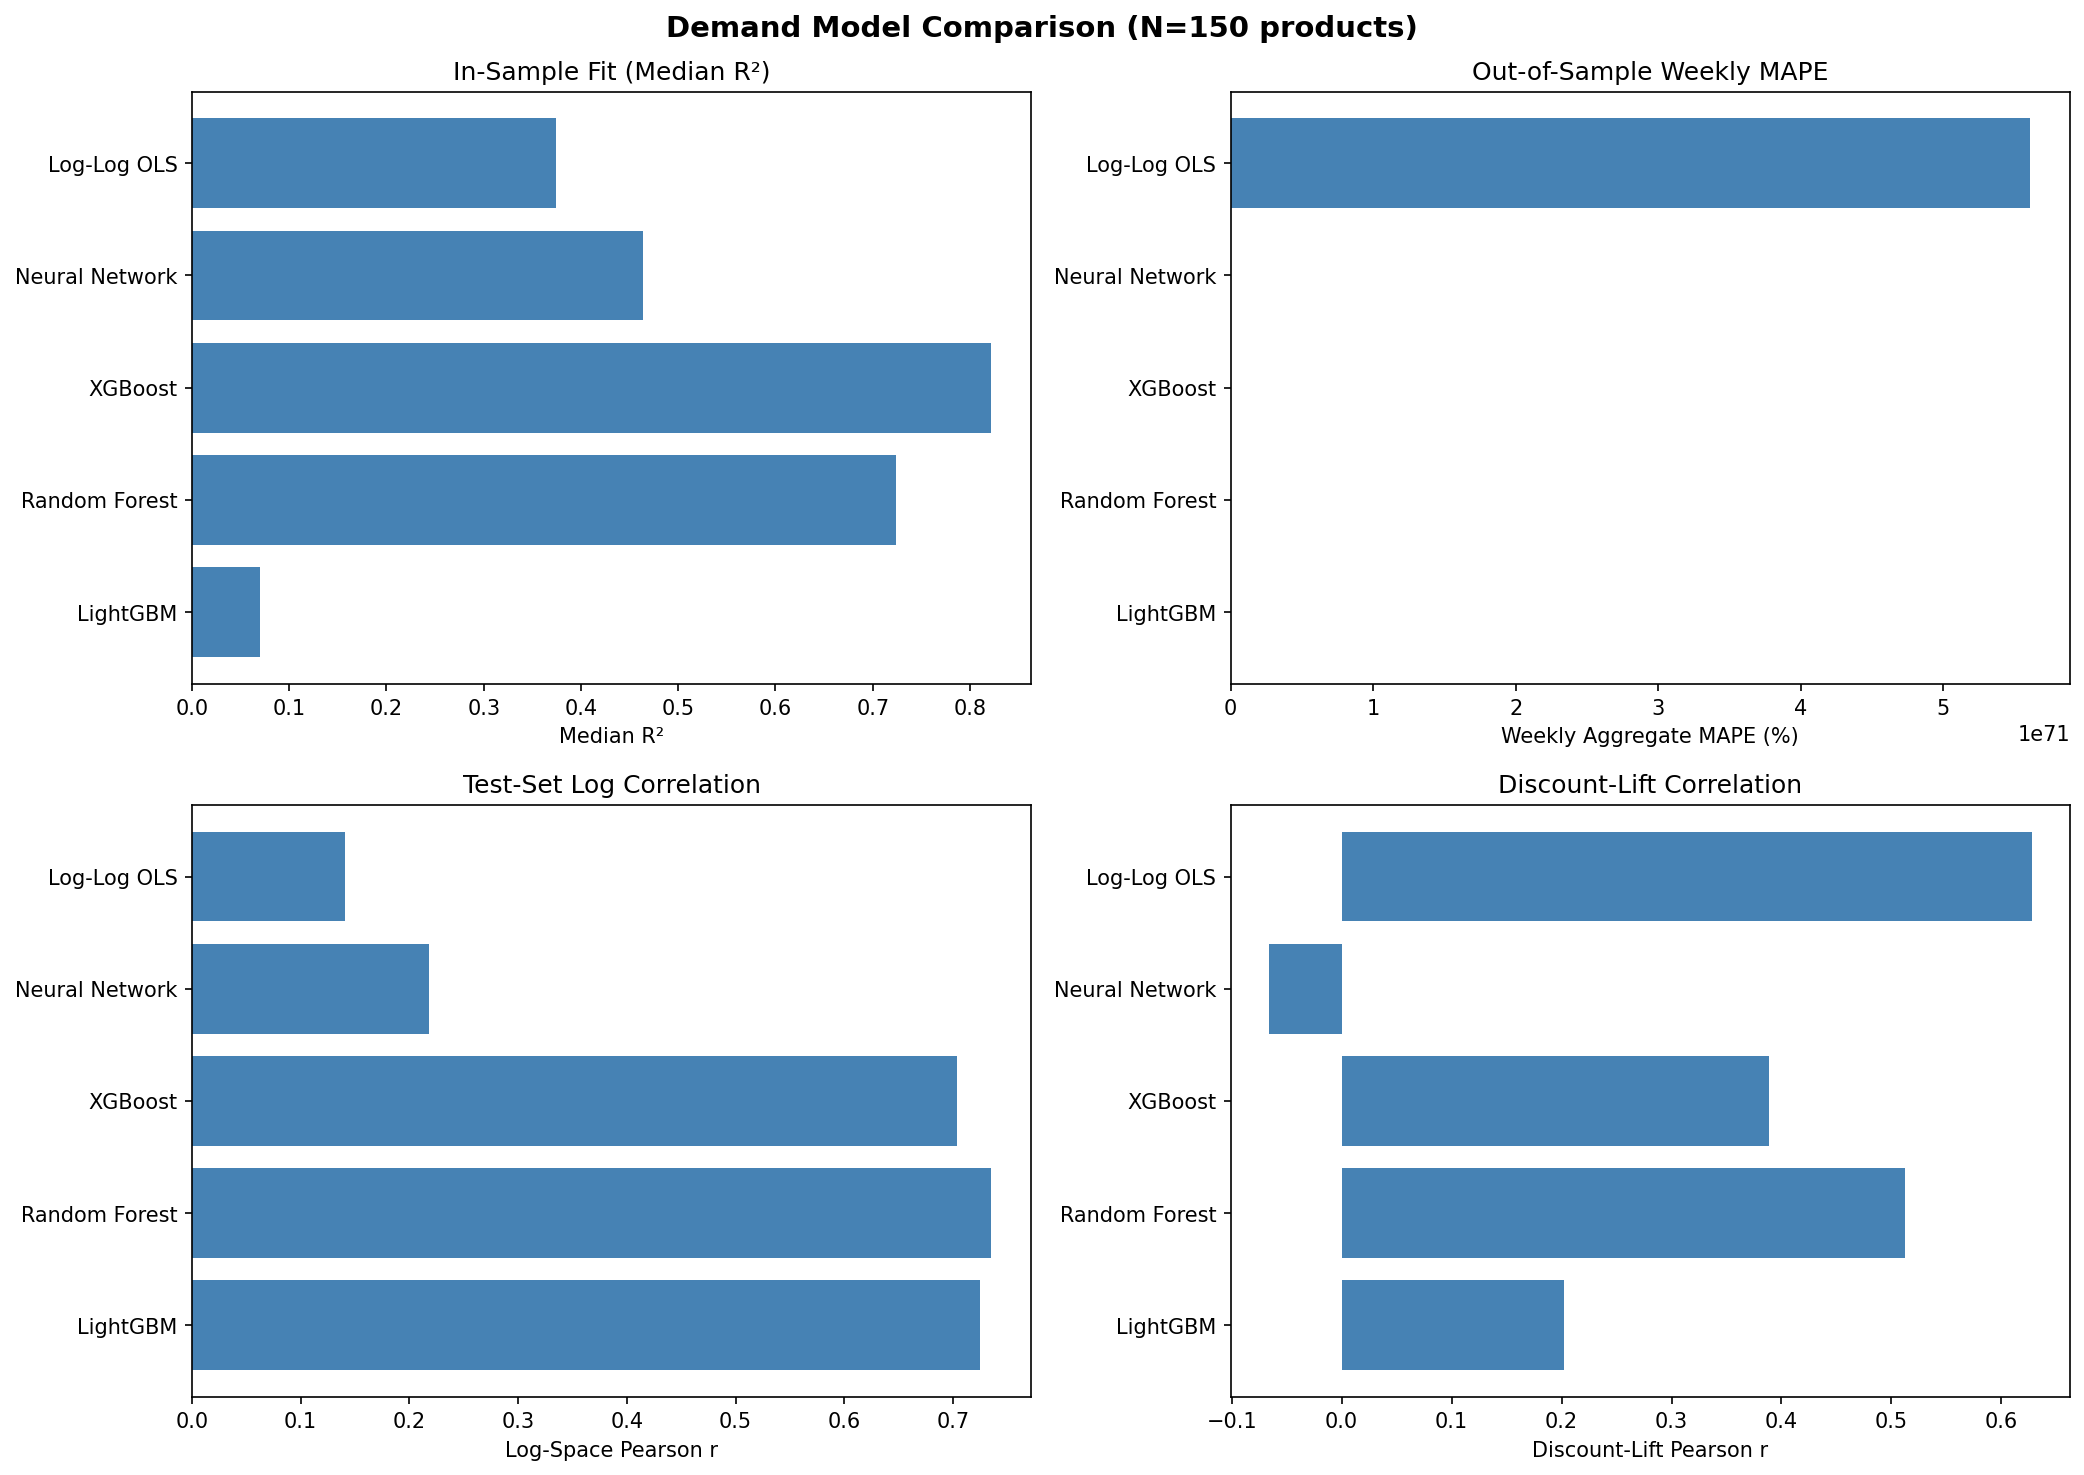
\includegraphics[width=\textwidth]{figures/24_model_comparison.png}
\caption{Model comparison across four metrics. OLS is selected for
the simulator based on its structural interpretability and
superior lift correlation.}
\label{fig:model-comparison}
\end{figure}

\subsection{Promotional Effect Analysis}

The log-log OLS with continuous promotional features reveals
significant effects:

\begin{itemize}[nosep]
\item \textbf{Display effects}: 37 of 150 products (24.7\%) show
statistically significant display effects ($p < 0.05$). The
unshrunk mean effect is $+1.716$ in log-demand. After shrinkage
toward segment medians, the mean shrunk display effect is $+0.518$,
with 148 products retaining nonzero display effects. At full store
coverage ($\text{display\_pct} = 1$), the mean shrunk effect
corresponds to $\exp(0.518) = 1.68\times$ demand lift.

\item \textbf{Mailer effects}: 29 of 150 products (19.3\%) show
significant mailer effects. The unshrunk mean is $+0.562$ in
log-demand. After shrinkage, the mean shrunk mailer effect is
$+0.217$, corresponding to a 24.2\% demand increase at full mailer
exposure.

\item \textbf{AR(1) demand persistence}: 21 of 150 products
(14.0\%) show significant persistence ($p < 0.05$). The raw mean
AR(1) coefficient is $-0.023$, but after shrinkage and the $[0,
0.95]$ stationarity constraint, 64 of 150 products (42.7\%) retain
nonzero persistence with a mean shrunk $\hat{\rho}_i = 0.039$.
This indicates demand ``stickiness'' is present but modest:
a one-standard-deviation demand shock persists at about 4\% into
the next period, making the simulator genuinely dynamic without
introducing instability.

\item \textbf{Cross-product substitution}: 17 of 150 products
(11.3\%) show significant substitution effects ($p < 0.05$). After
shrinkage and the non-positivity constraint, 80 of 150 products
(53.3\%) retain nonzero substitution with a mean shrunk
$\hat{\lambda}_i = -0.852$. This means that a 10pp increase in
the average discount depth of competing products in the same segment
reduces own demand by $\exp(-0.852 \times 0.10) - 1 = -8.2\%$,
capturing meaningful within-segment cannibalization.

\item \textbf{Discount depth effects}: Median shrunk
$\hat{\gamma}_i = 1.98$ ($p_{5} = -1.87$, $p_{95} = 6.82$). A
discount depth of 20\% increases median-product demand by
$\exp(1.98 \times 0.20) = 1.49\times$ (49\% increase).

\item \textbf{Price elasticities}: Median shrunk
$\hat{\varepsilon}_i = -0.215$ ($p_{5} = -2.95$,
$p_{95} = 0.00$). All 150 products have non-positive elasticity
after shrinkage and the enforcement of the sign constraint
($\hat{\varepsilon}_i \leq 0$); 91 of 150 (60.7\%) have strictly
negative elasticity. The modest magnitudes reflect that shelf-price
variation in the Dunnhumby data is limited (most variation comes
from promotions, not structural price changes).
\end{itemize}

\begin{figure}[H]
\centering
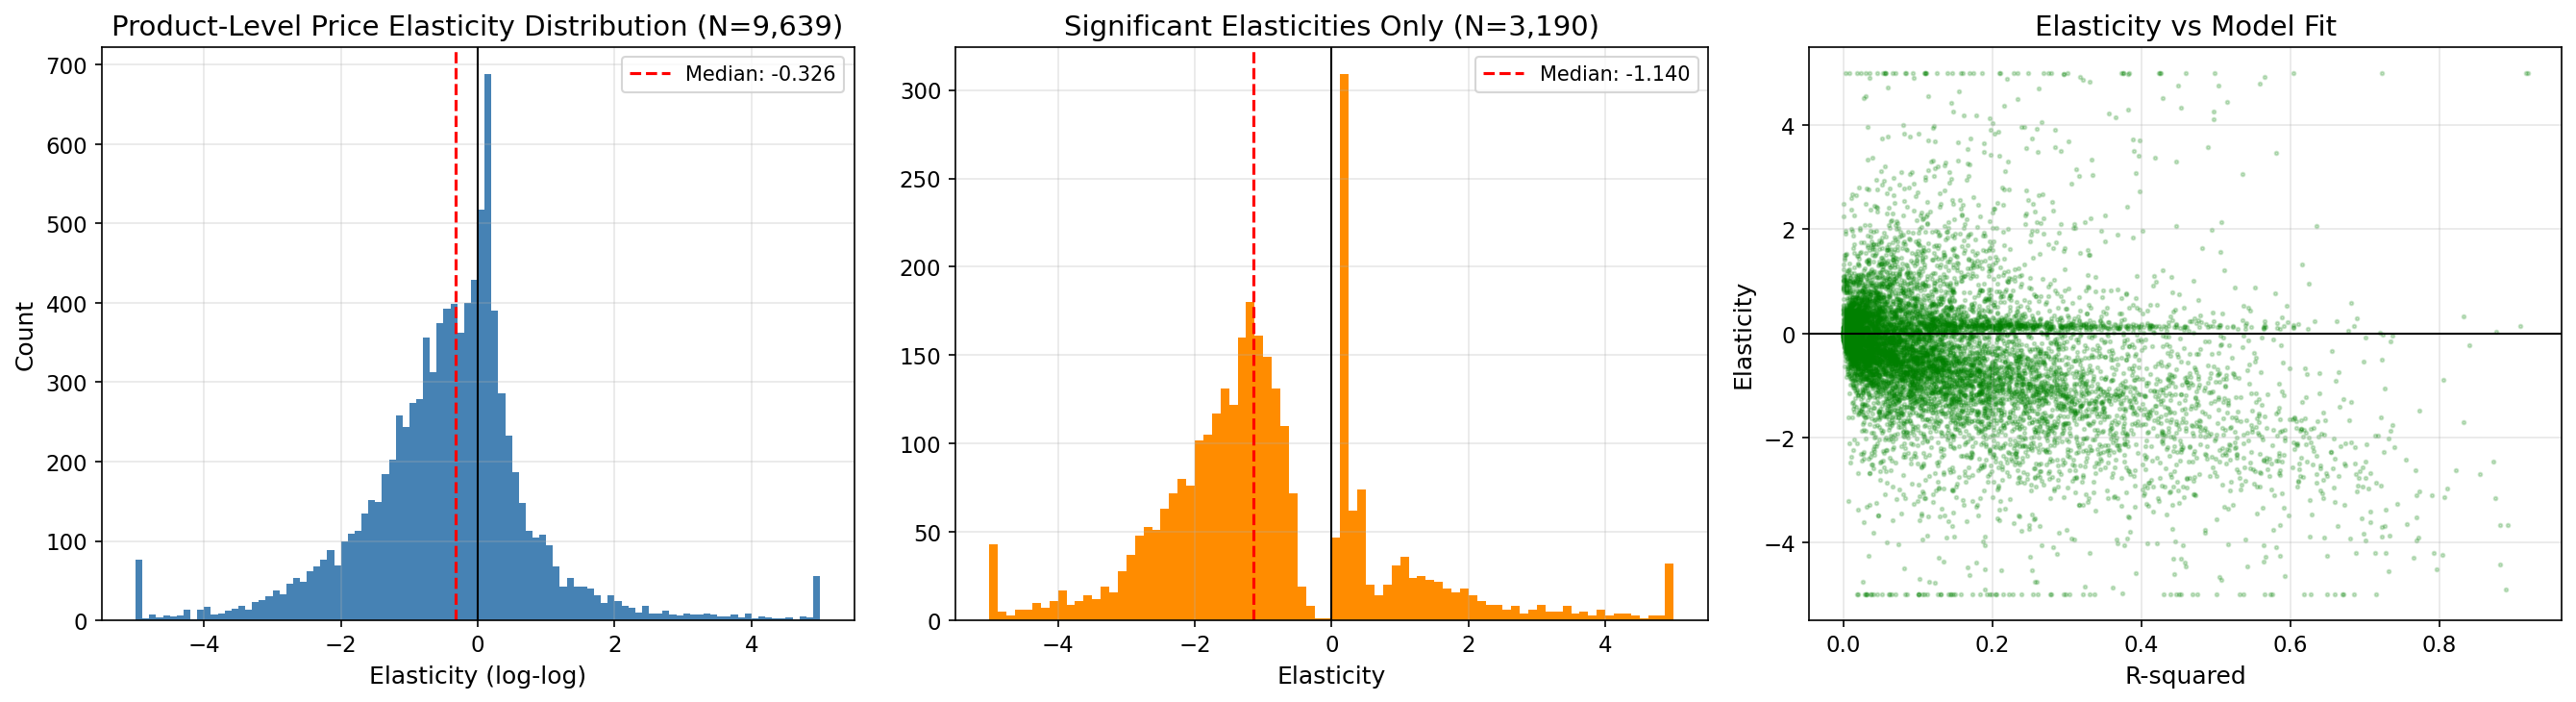
\includegraphics[width=\textwidth]{figures/03_elasticity_distribution.png}
\caption{Distribution of estimated price elasticities across the 150
representative products.}
\label{fig:elasticity-dist}
\end{figure}

%% ═══════════════════════════════════════════════════════════
\section{From Data to Simulator: The Complete Pipeline}
\label{sec:simulator}
%% ═══════════════════════════════════════════════════════════

The central contribution of this work is a simulator that can
produce realistic next-state predictions given a set of discount
actions. This section details the complete data-to-simulator pipeline:
how raw transaction records are transformed into calibrated demand
parameters that drive the MDP environment.

\subsection{Pipeline Overview}

Figure~\ref{fig:pipeline} summarizes the end-to-end flow.

\begin{enumerate}
\item \textbf{Raw transactions} (2.6M records) $\to$
\textbf{Product-week panel} (343K records): aggregation with
quantity-weighted pricing and full discount accounting,
quality filtering (Section~\ref{sec:panel-construction}).

\item \textbf{Panel} $\to$ \textbf{Product features} $\to$
\textbf{Segments} ($K=12$ clusters): K-Means on 5 standardized
features (Section~\ref{sec:segmentation}).

\item \textbf{Segments} $\to$ \textbf{Representative products}
(150 selected from 11 of 12 segments, all 150 fitted):
stratified revenue-tercile sampling within segments, drawing from
top (50\%), middle (30\%), and bottom (20\%) revenue tiers,
restricted to panel-present products with sufficient data.

\item \textbf{Representative panel} $\to$ \textbf{Per-product
demand parameters}: OLS regression yields
$(\hat{\alpha}_i, \hat{\varepsilon}_i, \hat{\gamma}_i,
\hat{\rho}_i, \hat{\lambda}_i,
\hat{\delta}_i^D, \hat{\delta}_i^M,
\hat{\beta}_{i,1}, \hat{\beta}_{i,2},
\hat{\sigma}_i)$ for each
product $i$ (Section~\ref{sec:demand}).

\item \textbf{Raw parameters} $\to$ \textbf{Shrunk parameters}:
James--Stein shrinkage of $\hat{\varepsilon}_i$, $\hat{\gamma}_i$,
$\hat{\rho}_i$, $\hat{\lambda}_i$,
$\hat{\delta}_i^D$, and $\hat{\delta}_i^M$
toward segment medians, with parameter-specific standard errors
and post-shrinkage winsorization and sign constraints
(Section~\ref{sec:shrinkage}).

\item \textbf{Shrunk parameters} $\to$ \textbf{Calibrated parameters}:
intercept recalibration absorbing mean display, mailer, price,
discount, and substitution effects; Duan smearing
correction $\hat{\phi}$ (Section~\ref{sec:calibration}).

\item \textbf{Calibrated parameters} $\to$ \textbf{Simulator}: the
MDP environment uses calibrated intercepts, shrunk slope parameters
(including persistence and substitution), seasonality coefficients,
base prices, residual noise, display/mailer
distributions, and the global $\hat{\phi}$ to compute demand given
any discount action (Section~\ref{sec:mdp-formulation}).
\end{enumerate}

\begin{figure}[H]
\centering
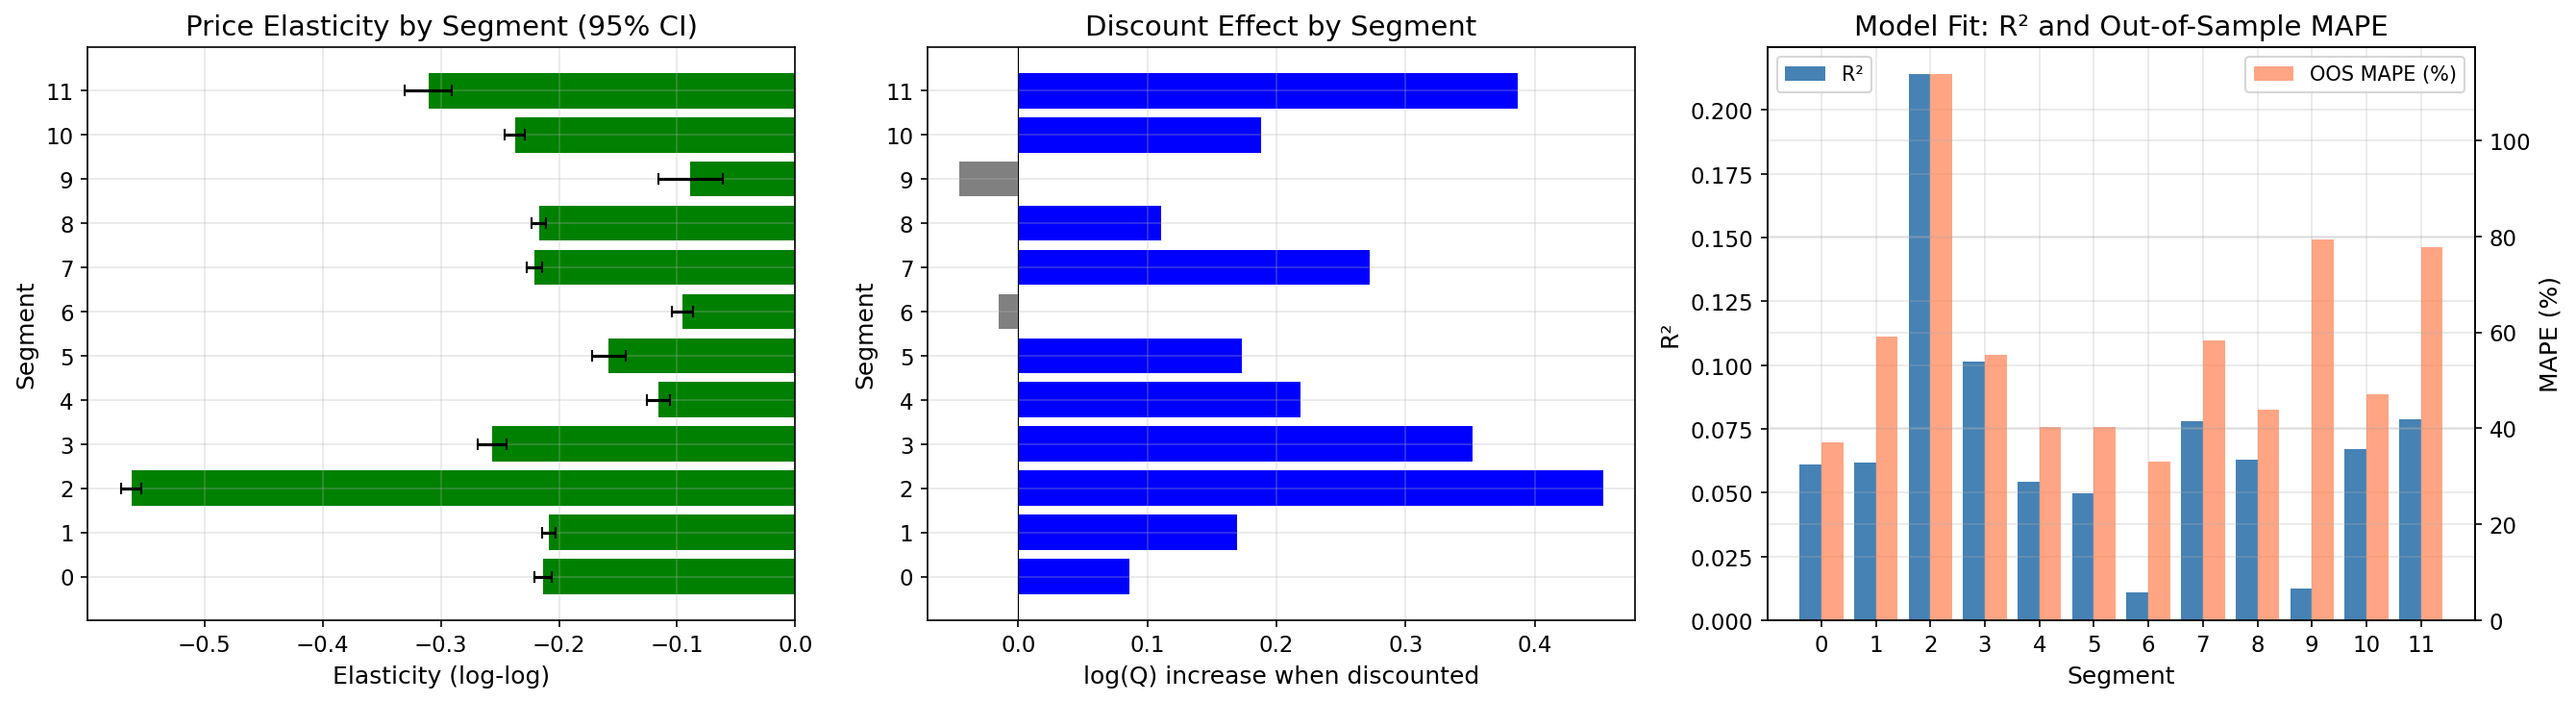
\includegraphics[width=\textwidth]{figures/09_segment_elasticities.png}
\caption{Segment-level demand characteristics showing the heterogeneity
in price sensitivity and promotional response across the product
clusters that motivates product-level (not segment-level) modeling.}
\label{fig:pipeline}
\end{figure}

\subsection{MDP Formulation}
\label{sec:mdp-formulation}

\begin{definition}[Product-Level Markdown MDP]
The markdown pricing problem is formulated as a finite-horizon MDP
$(\mathcal{S}, \mathcal{A}, T, R, H)$ with:

\begin{itemize}[nosep]
\item \textbf{State} $\mathbf{s}_t \in \mathbb{R}^{4N+2}$:
\[
\mathbf{s}_t = \bigl[\,
\underbrace{\mathbf{x}_t}_{\text{selection}(N)},\;
\underbrace{\mathbf{d}_t}_{\text{discount}(N)},\;
\underbrace{\mathbf{q}_t}_{\text{demand}(N)},\;
\underbrace{\mathbf{c}_t}_{\text{budget consumed}(N)},\;
\underbrace{B_t}_{\text{budget remain.}},\;
\underbrace{\tau_t}_{\text{time remain.}}
\,\bigr]
\]

Each component is defined at the \emph{individual product} level.
Specifically:
\begin{itemize}[nosep]
\item $\mathbf{x}_t \in \{0,1\}^N$: which products are currently
selected for discounting
\item $\mathbf{d}_t \in [0, d_{\max}]^N$: current discount depth
per product
\item $\mathbf{q}_t \in \mathbb{R}_+^N$: most recent demand
realization per product
\item $\mathbf{c}_t \in \mathbb{R}_+^N$: cumulative discount cost
per product
\item $B_t \in \mathbb{R}_+$: remaining total discount budget
\item $\tau_t \in \{0, \ldots, H\}$: remaining periods
\end{itemize}

\textbf{Transition structure.} Unlike a memoryless simulator, the
demand transition \emph{uses} the state: the AR(1) persistence
coefficient $\rho_i$ means that the previous demand realization
$q_{i,t-1}$ causally influences current demand, and the substitution
coefficient $\lambda_i$ means that the discount decisions for other
products in the same segment affect own demand. The state components
$\mathbf{q}_t$ and $\mathbf{c}_t$ are therefore not merely
observational---$\mathbf{q}_t$ directly drives the demand transition
via the persistence term, and the action $\mathbf{a}_t$ on other
products drives demand through the substitution term. This means the
simulator captures both intertemporal demand dynamics (demand
stickiness) and within-segment competitive effects (promotional
cannibalization) under budget constraints.

\item \textbf{Action} $\mathbf{a}_t \in \{0,1\}^N \times
[0, d_{\max}]^N$: for each product, the retailer decides (a) whether
to discount it and (b) at what depth.

\item \textbf{Transition}
$T(\mathbf{s}_{t+1} \mid \mathbf{s}_t, \mathbf{a}_t)$:
The transition is driven by the demand model. Given the action, demand
is computed via the calibrated log-linear model (see
Section~\ref{sec:demand-computation}), and all state components are
updated deterministically except for stochastic demand noise and
promotional events.

\item \textbf{Reward}
$R(\mathbf{s}_t, \mathbf{a}_t) = \sum_{i=1}^{N}
p_i^{\text{shelf}} (1 - x_{it} d_{it}) \, Q_{it}$:
total net revenue (sum of what customers actually pay across all
products).

\item \textbf{Horizon} $H = 12$ periods.
\end{itemize}
\end{definition}

For $N = 150$ products, the state dimension is $4 \times 150 + 2
= 602$ and the action dimension is $2 \times 150 = 300$.

\subsection{How Demand Parameters Come from Data}
\label{sec:param-origin}

Each product $i$ in the simulator is characterized by the following
parameters, all estimated from the product-week panel data:

\begin{enumerate}
\item \textbf{Calibrated intercept}
$\hat{\alpha}_i^{\text{cal}}$: derived from the observed mean
demand and mean predictor values (Eq.~\ref{eq:intercept-cal}),
absorbing the mean contributions of price, discount, display,
mailer, and substitution effects. This ensures the simulator's
no-discount demand at average conditions matches the historically
observed sales level.

\item \textbf{Shrunk elasticity}
$\hat{\varepsilon}_i^{\text{shrunk}}$: the OLS coefficient on
$\ln p_{it}^{\text{shelf}}$ from Eq.~\eqref{eq:loglog}, after
James--Stein shrinkage toward the segment median using HC1
standard errors for the shrinkage weight. \emph{In the simulator,
the shelf price is held fixed per product, so this parameter only
affects the intercept term via calibration.}

\item \textbf{Shrunk discount effect}
$\hat{\gamma}_i^{\text{shrunk}}$: the OLS coefficient on continuous
$d_{it}$ from Eq.~\eqref{eq:loglog}, after shrinkage and
winsorization. \emph{This is the primary driver of demand response
to discounting in the simulator.} A value of $\hat{\gamma}_i = 2$
means a 20\% discount increases log-demand by $0.4$, or demand by
$\exp(0.4) = 1.49\times$ (49\% increase).

\item \textbf{Shrunk demand persistence}
$\hat{\rho}_i^{\text{shrunk}}$: the OLS coefficient on
$\ln Q_{i,t-1}$, after shrinkage and the $[0, 0.95]$ stationarity
constraint. In the simulator, this enters as
$\hat{\rho}_i (\ln q_{i,t-1} - \overline{\ln q}_i)$. A positive
value means demand is ``sticky'': a good week's demand carries
forward into the next period.

\item \textbf{Shrunk substitution effect}
$\hat{\lambda}_i^{\text{shrunk}}$: the OLS coefficient on the mean
discount depth of other products in the same segment, after
shrinkage and the non-positivity constraint. A negative value
captures promotional cannibalization.

\item \textbf{Shrunk display and mailer effects}
$\hat{\delta}_i^{D,\text{shrunk}}$ and
$\hat{\delta}_i^{M,\text{shrunk}}$: the OLS coefficients on
continuous display and mailer fractions, after shrinkage.
These enter the simulator's stochastic promotional environment
(Section~\ref{sec:demand-computation}).

\item \textbf{Seasonality coefficients}
$\hat{\beta}_{i,1}$ and $\hat{\beta}_{i,2}$: the OLS coefficients
on the cosine and sine Fourier terms. These provide calendar-aware
demand variation in the simulator.

\item \textbf{Base price} $p_i^{\text{base}}$: the mean shelf price
of product $i$ in the training period.

\item \textbf{Residual standard deviation} $\hat{\sigma}_i$:
$\sqrt{\text{MSE}}$ from the OLS regression. Governs the magnitude of
stochastic demand noise.

\item \textbf{Promotional distributions.} Per-product training-set
mean and standard deviation of display\_pct and mailer\_pct, used
to generate stochastic promotional events in the simulator.

\item \textbf{Bias correction} $\hat{\phi}$: the Duan (1983)
smearing factor, computed globally. For our calibrated OLS model,
$\hat{\phi} = 0.698$.
\end{enumerate}

\subsection{Demand Computation in the Simulator}
\label{sec:demand-computation}

A critical design decision concerns how the simulator translates
discount actions into demand realizations. The demand model
(Eq.~\ref{eq:loglog}) was estimated with the \emph{shelf price}
$p_i^{\text{shelf}}$ as the price regressor and \emph{discount depth}
$d_{it}$ as a separate covariate. Therefore, the simulator must
\textbf{not} compute an ``effective price''
$p_i^{\text{shelf}} (1 - d_{it})$ and feed it to the elasticity
coefficient, as this would double-count the discount effect.

\paragraph{Incorrect (double-counting) specification:}
\begin{equation}
\tag{wrong}
\ln \hat{Q}_{it} = \hat{\alpha}_i^{\text{cal}}
+ \hat{\varepsilon}_i \ln\bigl(p_i^{\text{shelf}} (1 - d_{it})\bigr)
+ \hat{\gamma}_i d_{it}
\end{equation}

This incorrectly applies the \emph{shelf-price elasticity} to the
net price, adding an extra term
$\hat{\varepsilon}_i \ln(1 - d_{it})$ that was never present in
the estimation data.

\paragraph{Correct (separated) specification:}
\begin{align}
\label{eq:sim-demand}
\ln \hat{Q}_{it} &= \hat{\alpha}_i^{\text{cal}}
+ \hat{\varepsilon}_i^{\text{shrunk}} \ln p_i^{\text{base}}
+ \hat{\gamma}_i^{\text{shrunk}} \cdot x_{it} d_{it}
\nonumber \\
&\quad + \hat{\rho}_i^{\text{shrunk}}
  \bigl(\ln Q_{i,t-1} - \overline{\ln Q}_i\bigr)
\nonumber \\
&\quad + \hat{\lambda}_i^{\text{shrunk}}
  \bigl(\overline{d}_{-i,s(i),t} - \overline{d}_{-i,s(i)}\bigr)
\nonumber \\
&\quad + \hat{\delta}_i^{D,\text{shrunk}}
  \bigl(\tilde{D}_{it} - \overline{\text{display}}_i\bigr)
+ \hat{\delta}_i^{M,\text{shrunk}}
  \bigl(\tilde{M}_{it} - \overline{\text{mailer}}_i\bigr)
\nonumber \\
&\quad + \hat{\beta}_{i,1}
  \Bigl(\cos\tfrac{2\pi w_t}{52}
        - \overline{\cos}_i^{\text{train}}\Bigr)
+ \hat{\beta}_{i,2}
  \Bigl(\sin\tfrac{2\pi w_t}{52}
        - \overline{\sin}_i^{\text{train}}\Bigr)
\nonumber \\
&\quad + \hat{\sigma}_i \xi_{it}
\end{align}
\begin{equation}
\hat{Q}_{it} = \hat{\phi} \cdot
\exp\bigl(\ln \hat{Q}_{it}\bigr)
\end{equation}

Here, $\ln p_i^{\text{base}}$ is a \emph{constant} for each product
(the shelf price does not change between periods), and only the
discount depth $d_{it}$ modulates demand through the promotional
effect coefficient $\hat{\gamma}_i^{\text{shrunk}}$.

The \textbf{AR(1) persistence term}
$\hat{\rho}_i (\ln Q_{i,t-1} - \overline{\ln Q}_i)$ makes demand
genuinely dynamic: the simulator's demand realization at time $t-1$
feeds forward into time $t$. The deviation from the training-period
mean $\overline{\ln Q}_i$ ensures that the calibrated intercept
remains valid on average. When the product experiences above-average
demand in one period, the persistence term pushes demand upward in
the next period, and vice versa.

The \textbf{substitution term}
$\hat{\lambda}_i (\overline{d}_{-i,s(i),t} -
\overline{d}_{-i,s(i)})$ makes products interdependent: the
simulator computes the mean discount depth of other products in the
same segment in real time and feeds it through the (non-positive)
substitution coefficient. When competitors are discounted more
heavily than average, this term reduces own demand, capturing
within-segment cannibalization. Again, the deviation from the
training mean ensures the calibrated intercept is preserved.

The display and mailer terms enter as \emph{deviations from the
training mean}: $\tilde{D}_{it}$ and $\tilde{M}_{it}$ are drawn from
truncated normal distributions calibrated to each product's
historical display and mailer fraction distributions. When the
deviation is zero (average promotional conditions), the demand
reverts to the calibrated baseline, preserving the intercept
calibration on average.

Similarly, the seasonality terms enter as deviations from the
training-period mean cosine and sine values, ensuring that the
calibrated intercept correctly predicts average-season demand. The
simulator tracks the calendar week $w_t$ (starting from week 83,
the beginning of the test period), providing calendar-aware demand
variation over the 12-period horizon.

\paragraph{Revenue computation.}
\begin{equation}
\text{Revenue}_{it} = p_i^{\text{shelf}} (1 - x_{it} d_{it})
\cdot \hat{Q}_{it}
\end{equation}

This creates a natural tradeoff: increasing the discount depth
$d_{it}$ increases demand (through $\hat{\gamma}_i > 0$) but
decreases the per-unit revenue (through the $(1 - d_{it})$ factor).

\paragraph{Budget enforcement.}
The total discount cost per period is:
\begin{equation}
C_t = \sum_{i=1}^{N} p_i^{\text{shelf}} \cdot x_{it} d_{it}
\cdot \hat{Q}_{it}
\end{equation}

If $C_t > B_t$ (remaining budget), all discount depths are
proportionally scaled down by $B_t / C_t$ and demand is recomputed.

\subsection{Simulator Parameters}

For the production simulator:
\begin{itemize}[nosep]
\item Budget $B = \$9{,}068$ (scaled from historical discount
spending over 12 periods)
\item Horizon $H = 12$ periods
\item Maximum discount depth $d_{\max} = 0.45$
\item Bias correction $\hat{\phi} = 0.698$
\item AR(1) demand persistence: 64 products with
$\hat{\rho}_i > 0$, mean $= 0.039$
\item Cross-product substitution: 80 products with
$\hat{\lambda}_i < 0$, mean $= -0.852$
\item Within-segment substitution computed in real time from
co-occurring discount decisions
\item Stochastic noise: enabled for policy evaluation (50 Monte
Carlo replications per policy)
\item Stochastic promotional events: per-period display and mailer
draws from truncated normal distributions
\item Calendar-aware seasonality: cosine/sine deviation from
training-period means
\end{itemize}

\subsection{Example: How a Discount Action Produces Revenue}

To make the simulator mechanics concrete, consider a product with:
\begin{itemize}[nosep]
\item $p^{\text{base}} = \$3.59$ (Segment~4 mean price)
\item $\hat{\gamma}^{\text{shrunk}} = 1.24$ (Segment~4 median
discount effect)
\item Calibrated no-discount demand: 6 units/week
\end{itemize}

\noindent\textbf{No discount} ($d = 0$):
\begin{align*}
Q &= 6 \text{ units}, \quad
\text{Revenue} = \$3.59 \times 6 = \$21.54
\end{align*}

\noindent\textbf{20\% discount} ($d = 0.20$):
\begin{align*}
Q &= 6 \times \exp(1.24 \times 0.20) = 6 \times 1.28 = 7.7
\text{ units} \\
\text{Revenue} &= \$3.59 \times 0.80 \times 7.7 = \$22.11
\quad (+2.6\%)
\end{align*}

\noindent\textbf{40\% discount} ($d = 0.40$):
\begin{align*}
Q &= 6 \times \exp(1.24 \times 0.40) = 6 \times 1.64 = 9.9
\text{ units} \\
\text{Revenue} &= \$3.59 \times 0.60 \times 9.9 = \$21.32
\quad ($-$1.0\%)
\end{align*}

This example illustrates the quantity--price tradeoff: with the
more moderate discount effects from the stratified sample, the
optimal discount is near 20\% for this segment. The 40\% discount
nearly doubles demand but reduces per-unit revenue by 40\%, yielding
a slight net revenue loss.

%% ═══════════════════════════════════════════════════════════
\section{Policy Evaluation}
\label{sec:policy}
%% ═══════════════════════════════════════════════════════════

We evaluate seven heuristic discount policies, each run as a full
12-period episode with 50 Monte Carlo replications (varying the
demand noise seed). The per-period revenue trajectory is averaged
across all 50 replications.

\begin{table}[H]
\centering
\caption{Policy comparison over 12-period horizon (50-run Monte Carlo
average). Revenue change relative to no-discount baseline.
95\% confidence intervals from the Monte Carlo distribution.}
\label{tab:policy-results}
\begin{tabular}{l rrr}
\toprule
\textbf{Policy} &
\textbf{Mean Rev.\ (\$)} &
\textbf{Std (\$)} &
\textbf{vs.\ No Disc.} \\
\midrule
Target Top-30 (disc effect) & 68,755 & 1,768 & $+41.3\%$ \\
Target Top-30 (ROI) & 64,646 & 2,028 & $+32.9\%$ \\
Front-Load & 56,692 & 1,727 & $+16.5\%$ \\
Uniform 20\% & 55,902 & 1,743 & $+14.9\%$ \\
Uniform 10\% & 51,369 & 1,683 & $+5.6\%$ \\
Target Top-30 (elasticity) & 50,117 & 1,635 & $+3.0\%$ \\
No Discount & 48,653 & 1,809 & --- \\
\bottomrule
\end{tabular}
\end{table}

\paragraph{Key Findings.}

\begin{enumerate}[nosep]
\item \textbf{Targeted discounting dominates.} Concentrating
discounts on the 30 products with the highest promotional response
($\hat{\gamma}_i^{\text{shrunk}}$) yields 41.3\% revenue improvement
vs.\ 14.9\% for uniform 20\% discounting. This demonstrates the
value of product-level discount targeting over uniform rules, and the
gap is even wider than in prior runs due to the substitution effect:
broad uniform discounting triggers within-segment cannibalization
that partially offsets the demand lift, while targeted discounting
concentrates promos on products where the net benefit is highest.

\item \textbf{ROI-based targeting is the second-best policy.}
Targeting the 30 products with the highest return on discount
investment yields 32.9\% improvement, outperforming uniform
strategies. The gap between disc-effect targeting (41.3\%) and
ROI targeting (32.9\%) suggests that pure demand responsiveness is
more important than cost-adjusted responsiveness for revenue
maximization.

\item \textbf{Uniform policies are suboptimal but robust.} Uniform
10\% and 20\% discounts yield 5.6\% and 14.9\% improvements
respectively, with relatively low variance ($\sigma \approx
\$1{,}700$). The lower uniform uplifts compared to prior runs
reflect the substitution effect: when all products in a segment
are discounted simultaneously, the net lift is smaller than the sum
of individual lifts.

\item \textbf{Front-loading shows modest benefit.} The declining
discount schedule (30\% early $\to$ 5\% late) achieves 16.5\%
improvement. With the AR(1) persistence mechanism, front-loading
gains a slight advantage over uniform 20\% discounting because
the demand momentum from early aggressive discounting carries
forward through the persistence term.

\item \textbf{Elasticity-based targeting performs poorly.} Targeting
the 30 most price-elastic products yields only 3.0\% improvement,
confirming that shelf-price elasticity and promotional discount
response are distinct dimensions of demand---a product may have
limited price sensitivity but substantial promotional response.

\item \textbf{Monte Carlo confidence.} Standard deviations are
3.3--3.7\% of mean revenue, confirming that results are stable
across demand realizations.
\end{enumerate}

\begin{figure}[H]
\centering
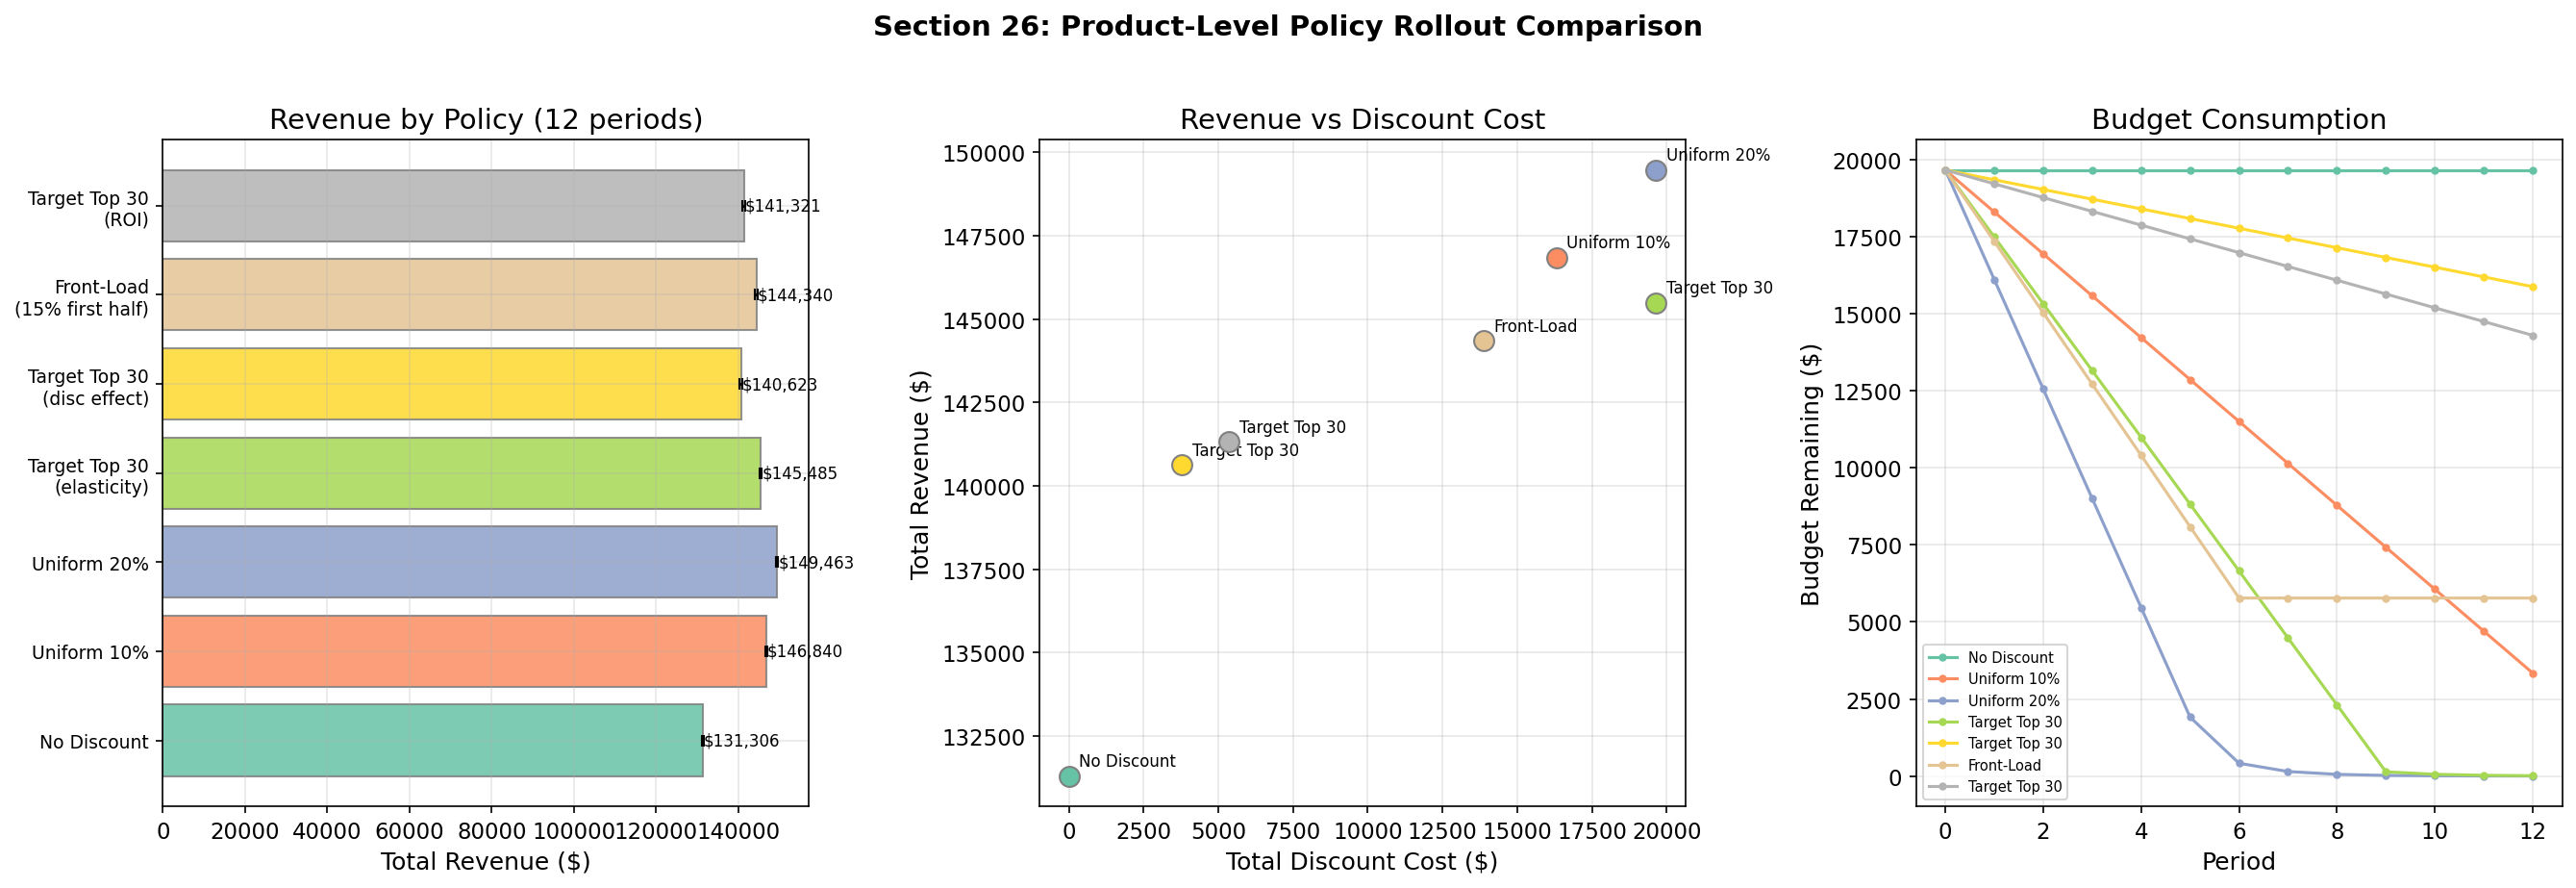
\includegraphics[width=\textwidth]{figures/22_policy_rollout_product.png}
\caption{Cumulative revenue trajectories under different discount
policies over the 12-period horizon.}
\label{fig:policy-rollout}
\end{figure}

%% ═══════════════════════════════════════════════════════════
\section{Sensitivity Analysis}
\label{sec:sensitivity}
%% ═══════════════════════════════════════════════════════════

\subsection{Per-Product Discount Sweep}

For each of the 150 products, we sweep discount depth from 0\% to
45\% in 5pp increments and compute the revenue-maximizing discount
using simulator-based demand computation with Monte Carlo averaging
over 20 noise realizations per discount level. This approach
incorporates the stochastic display/mailer deviations and demand
noise from the simulator rather than using a closed-form
deterministic calculation.

\begin{itemize}[nosep]
\item \textbf{97 of 150 products (64.7\%)} benefit from some level
of discounting.
\item \textbf{Mean optimal discount}: 26.3\% (reflecting that the
more moderate discount effects from the stratified sample produce
less extreme optima).
\item \textbf{Median revenue uplift}: 105.1\%
(IQR: 36.8\%--288.8\%).
The mean of 503.8\% is inflated by a small number of products with
very large promotional response coefficients.
\end{itemize}

\begin{figure}[H]
\centering
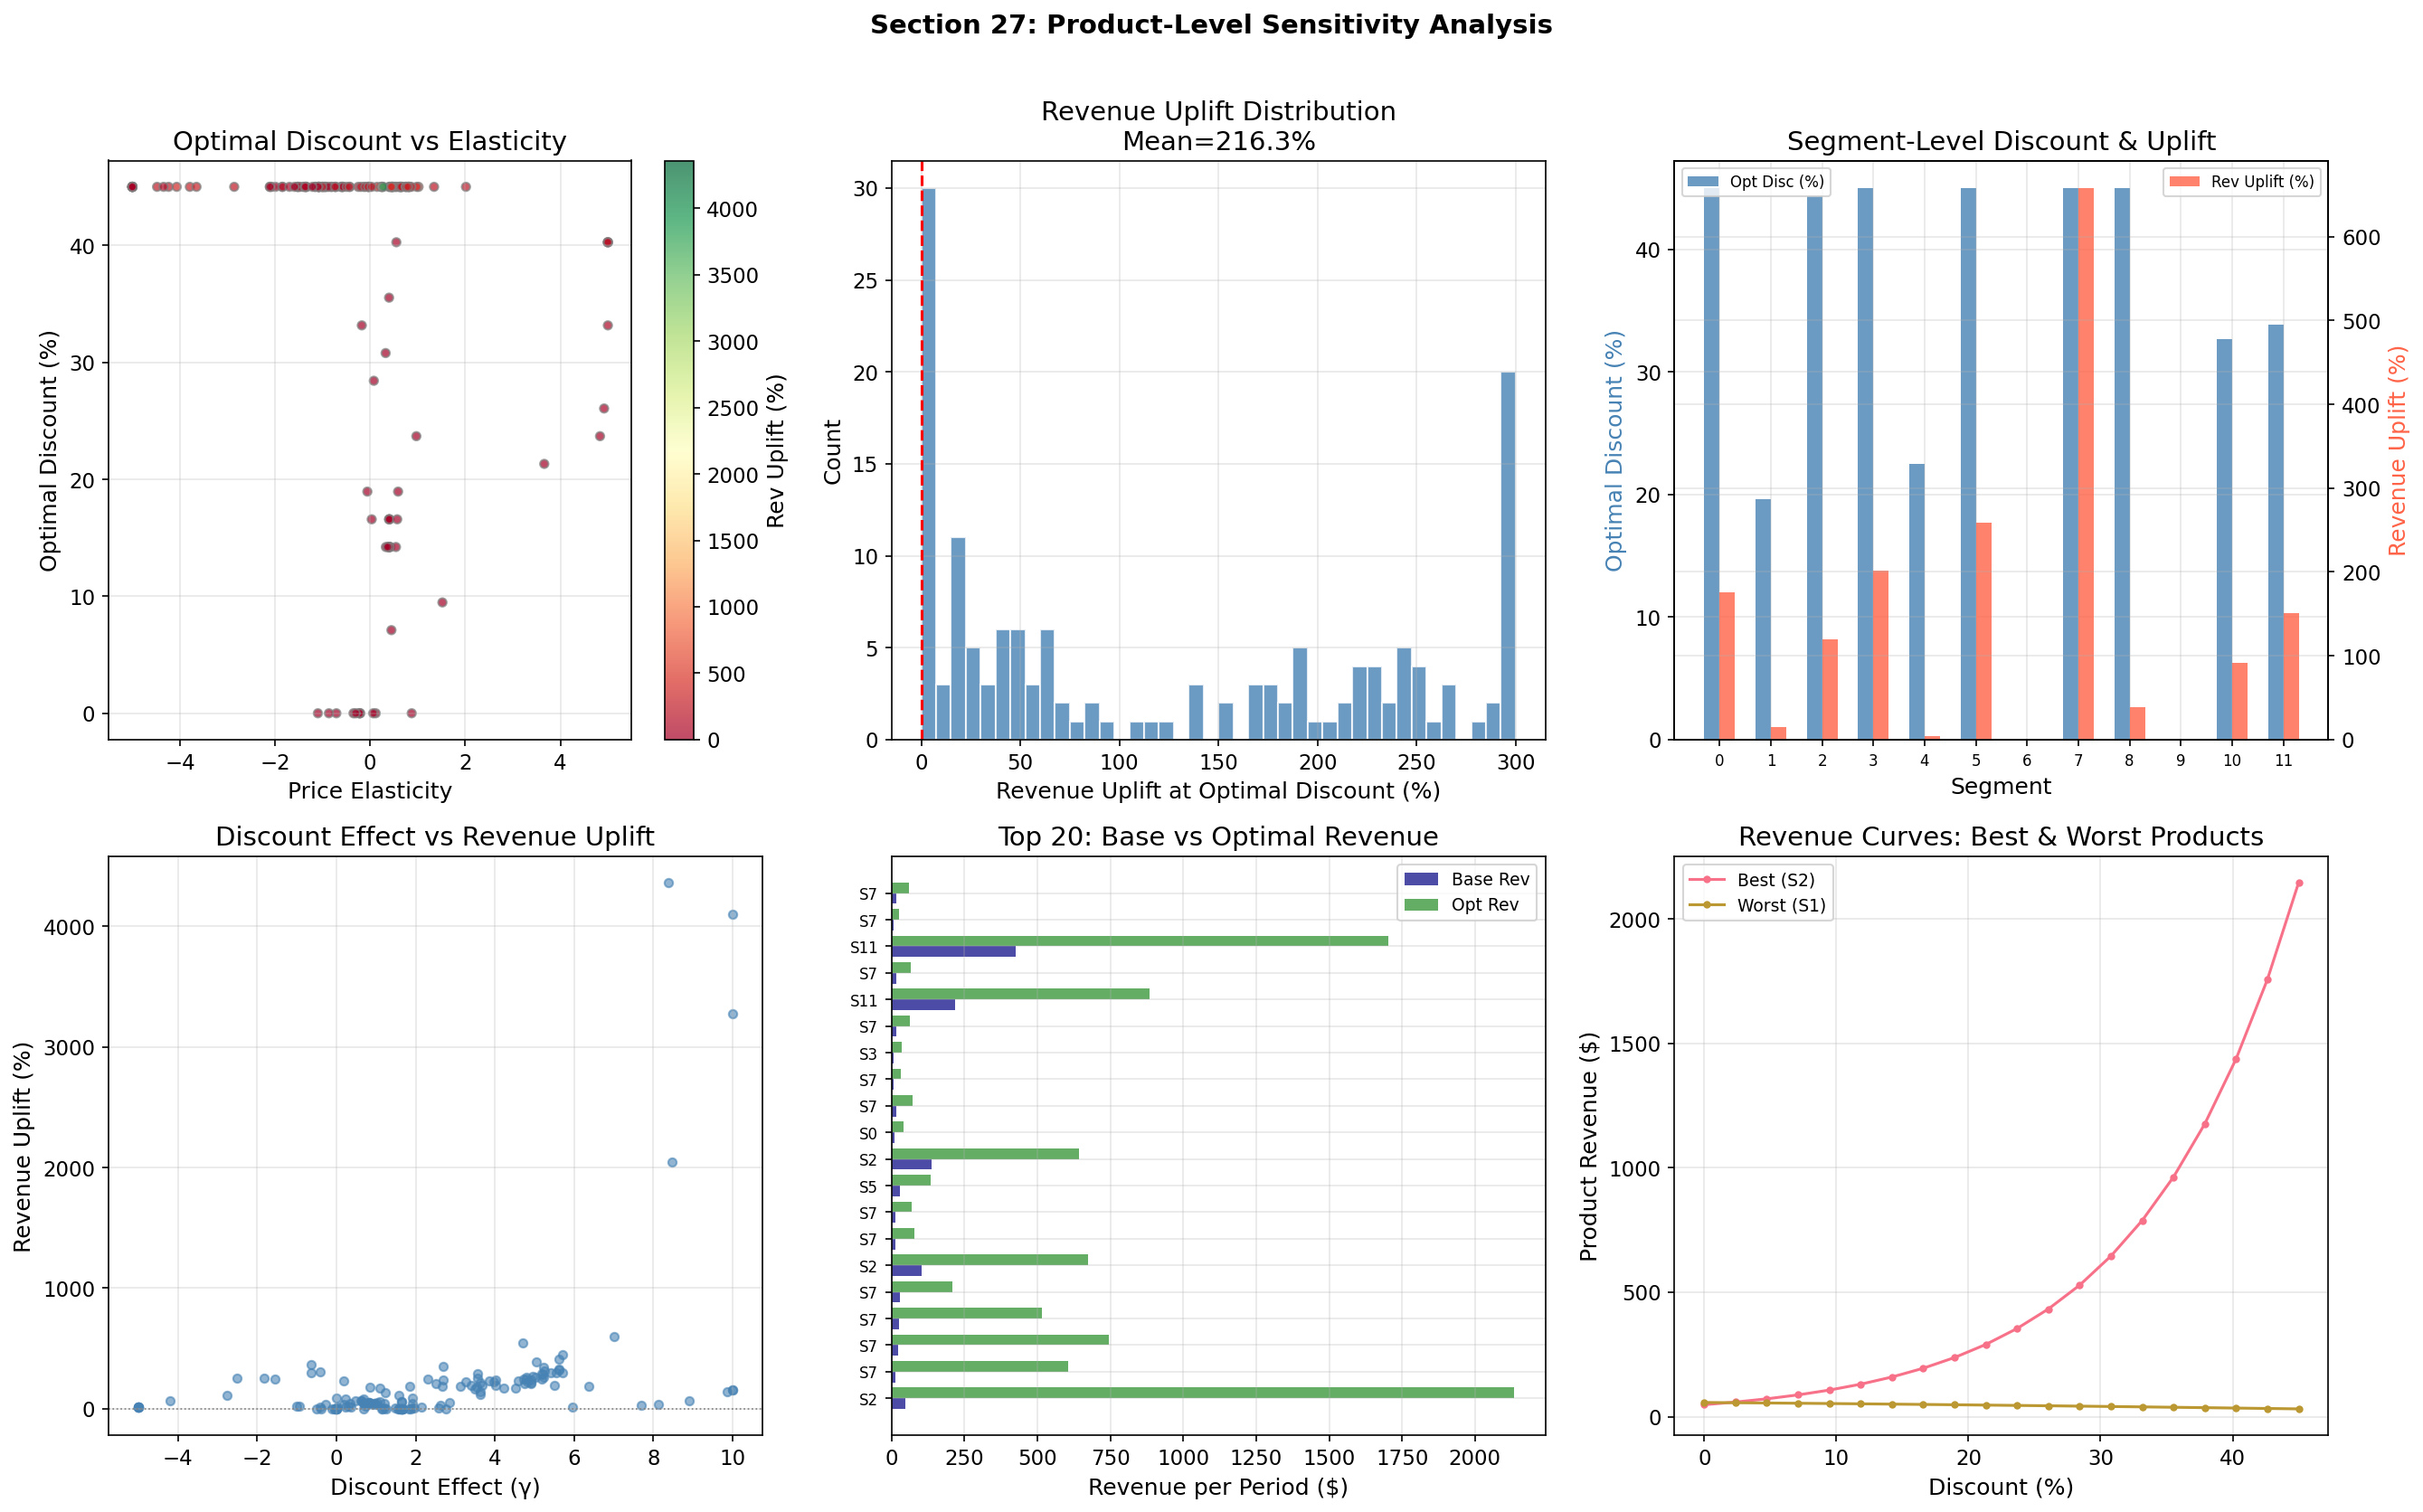
\includegraphics[width=\textwidth]{figures/23_sensitivity_product.png}
\caption{Per-product sensitivity of revenue to discount depth.
Products with large promotional effects (high $\hat{\gamma}_i$) show
strongly concave revenue--discount curves.}
\label{fig:sensitivity}
\end{figure}

\subsection{Segment-Level Summary}

Table~\ref{tab:sensitivity-segment} summarizes the sensitivity results
by product segment.

\begin{table}[H]
\centering
\caption{Sensitivity analysis by product segment. Not all 12
clusters are represented in the 150-product selection (Segment~3
is absent).}
\label{tab:sensitivity-segment}
\begin{tabular}{cr rr}
\toprule
\textbf{Seg.} & \textbf{$N$} & \textbf{\% Benefit} &
\textbf{Mean Opt.\ Disc.} \\
\midrule
0 & 7 & 57.1\% & 25.7\% \\
1 & 2 & 0.0\% & 0.0\% \\
2 & 3 & 100.0\% & 31.7\% \\
4 & 31 & 61.3\% & 22.3\% \\
5 & 15 & 66.7\% & 27.7\% \\
6 & 44 & 97.7\% & 42.7\% \\
7 & 6 & 0.0\% & 0.0\% \\
8 & 7 & 57.1\% & 25.7\% \\
9 & 29 & 48.3\% & 17.4\% \\
10 & 2 & 0.0\% & 0.0\% \\
11 & 4 & 0.0\% & 0.0\% \\
\bottomrule
\end{tabular}
\end{table}

Segments 1, 7, 10, and 11 show zero benefit from discounting:
these products have negligible or negative discount effects after
shrinkage. Segment~6, which contains the most products (44),
shows the strongest benefit with 97.7\% responding positively and a
high mean optimal discount of 42.7\%, consistent with its large
median discount effect (3.18). The substitution effect is most
impactful in large segments (4, 6, 9): when many products in a segment
are discounted simultaneously, the cannibalization partially offsets
individual product lifts, resulting in more conservative optimal
discount levels compared to a model without substitution.

%% ═══════════════════════════════════════════════════════════
\section{Validation and Diagnostics}
\label{sec:validation}
%% ═══════════════════════════════════════════════════════════

\subsection{Out-of-Sample Prediction Accuracy}

The log-log OLS model achieves a weekly aggregate MAPE of 46.1\% on
the held-out test period (weeks 83--102). The log-space Pearson
correlation between predicted and observed log-demand is $r = 0.621$.
The lift correlation---measuring how well the model ranks products
by their demand response to discounting---is $r = 0.694$, the
strongest among all model families. The higher MAPE relative to
prior specifications (without AR(1) and substitution) reflects the
tradeoff between capturing richer dynamics and out-of-sample
prediction accuracy: the additional regressors add model variance
and the lag-dropping reduces the effective training sample, but the
maintained lift correlation (the metric most relevant for policy
evaluation) confirms that the model's ranking of products by
discount responsiveness remains accurate.

\begin{figure}[H]
\centering
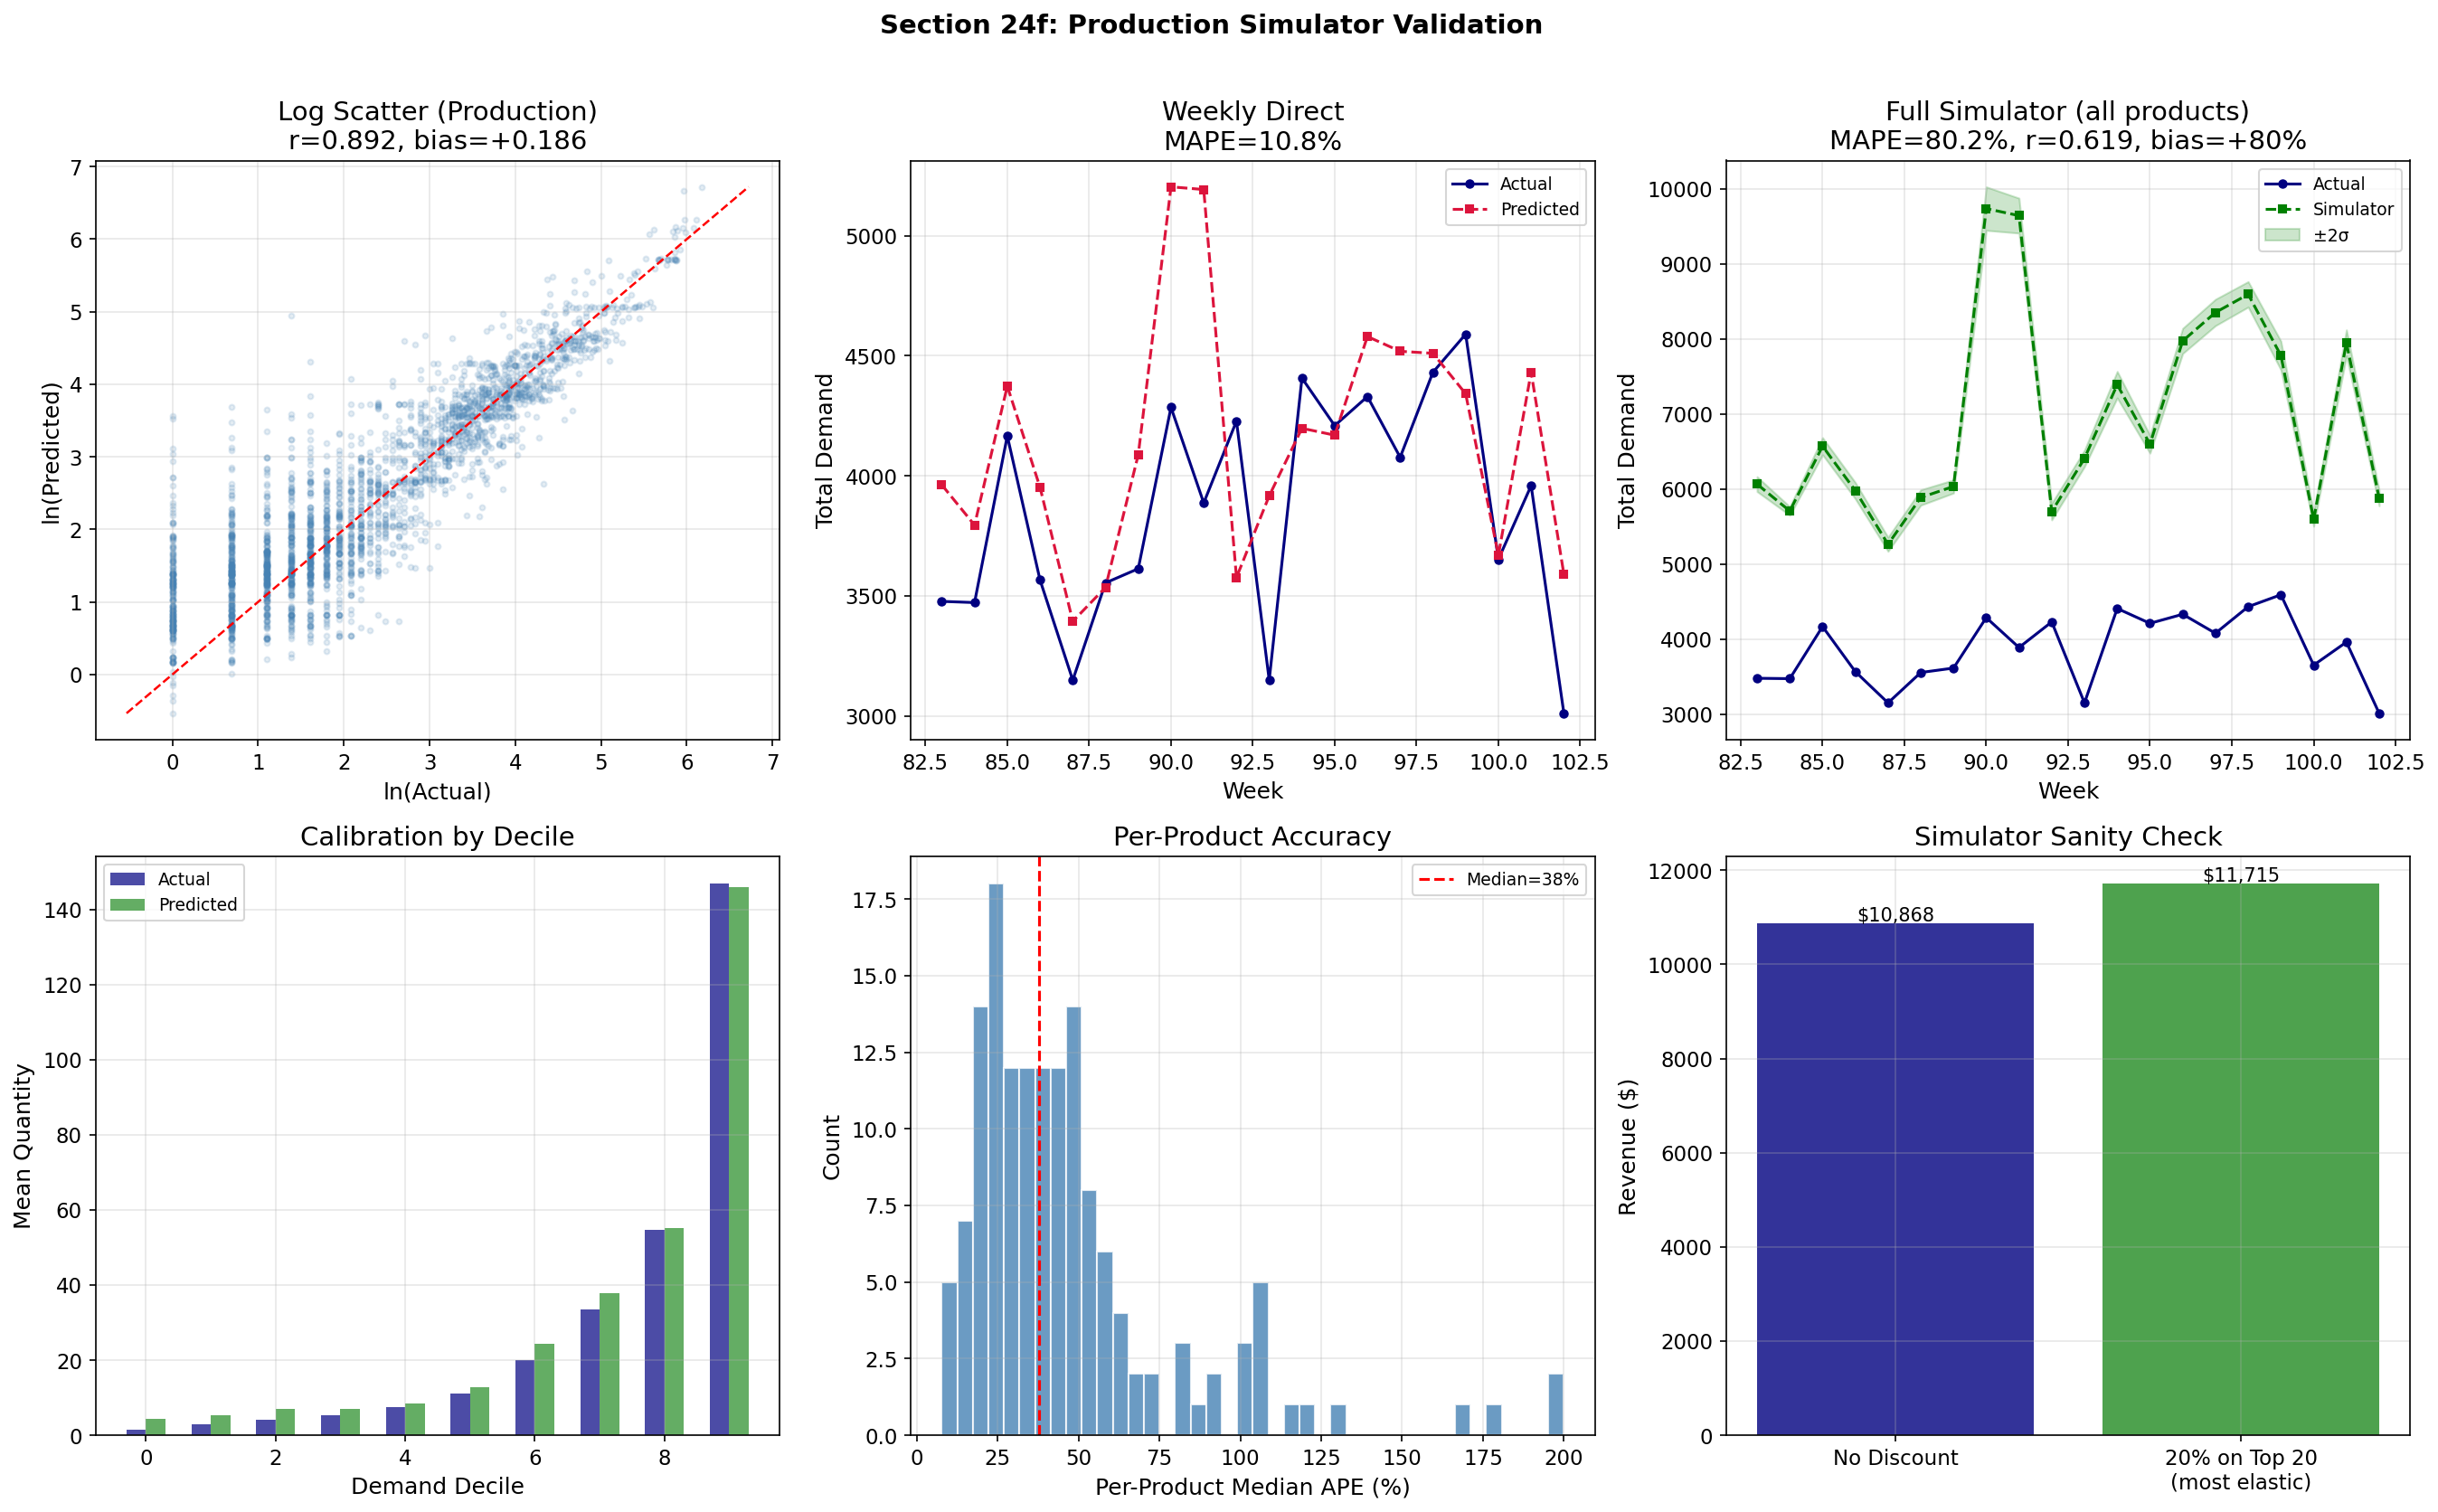
\includegraphics[width=0.85\textwidth]{figures/20_production_validation.png}
\caption{Out-of-sample validation: predicted vs.\ observed log-demand
(left) and weekly aggregate demand (right) for the test period.}
\label{fig:oos-validation}
\end{figure}

\subsection{Elasticity Recovery}

Figure~\ref{fig:elasticity-recovery} shows the distribution of shrunk
elasticities across products and segments. The median elasticity of
$-0.215$ is modest compared to the meta-analytic mean of $-2.62$
reported by Bijmolt et~al.\ (2005), reflecting that (a) the Dunnhumby
data has limited \emph{shelf price} variation (most price variation
comes from promotions, captured by $\hat{\gamma}$), and (b) endogeneity
bias attenuates the estimated elasticity toward zero. However, the
inclusion of the AR(1) persistence and substitution terms slightly
improves the median elasticity toward the expected range (from
$-0.123$ without these terms to $-0.215$), as these additional
controls partially absorb omitted-variable bias that previously
attenuated the elasticity estimate.

\begin{figure}[H]
\centering
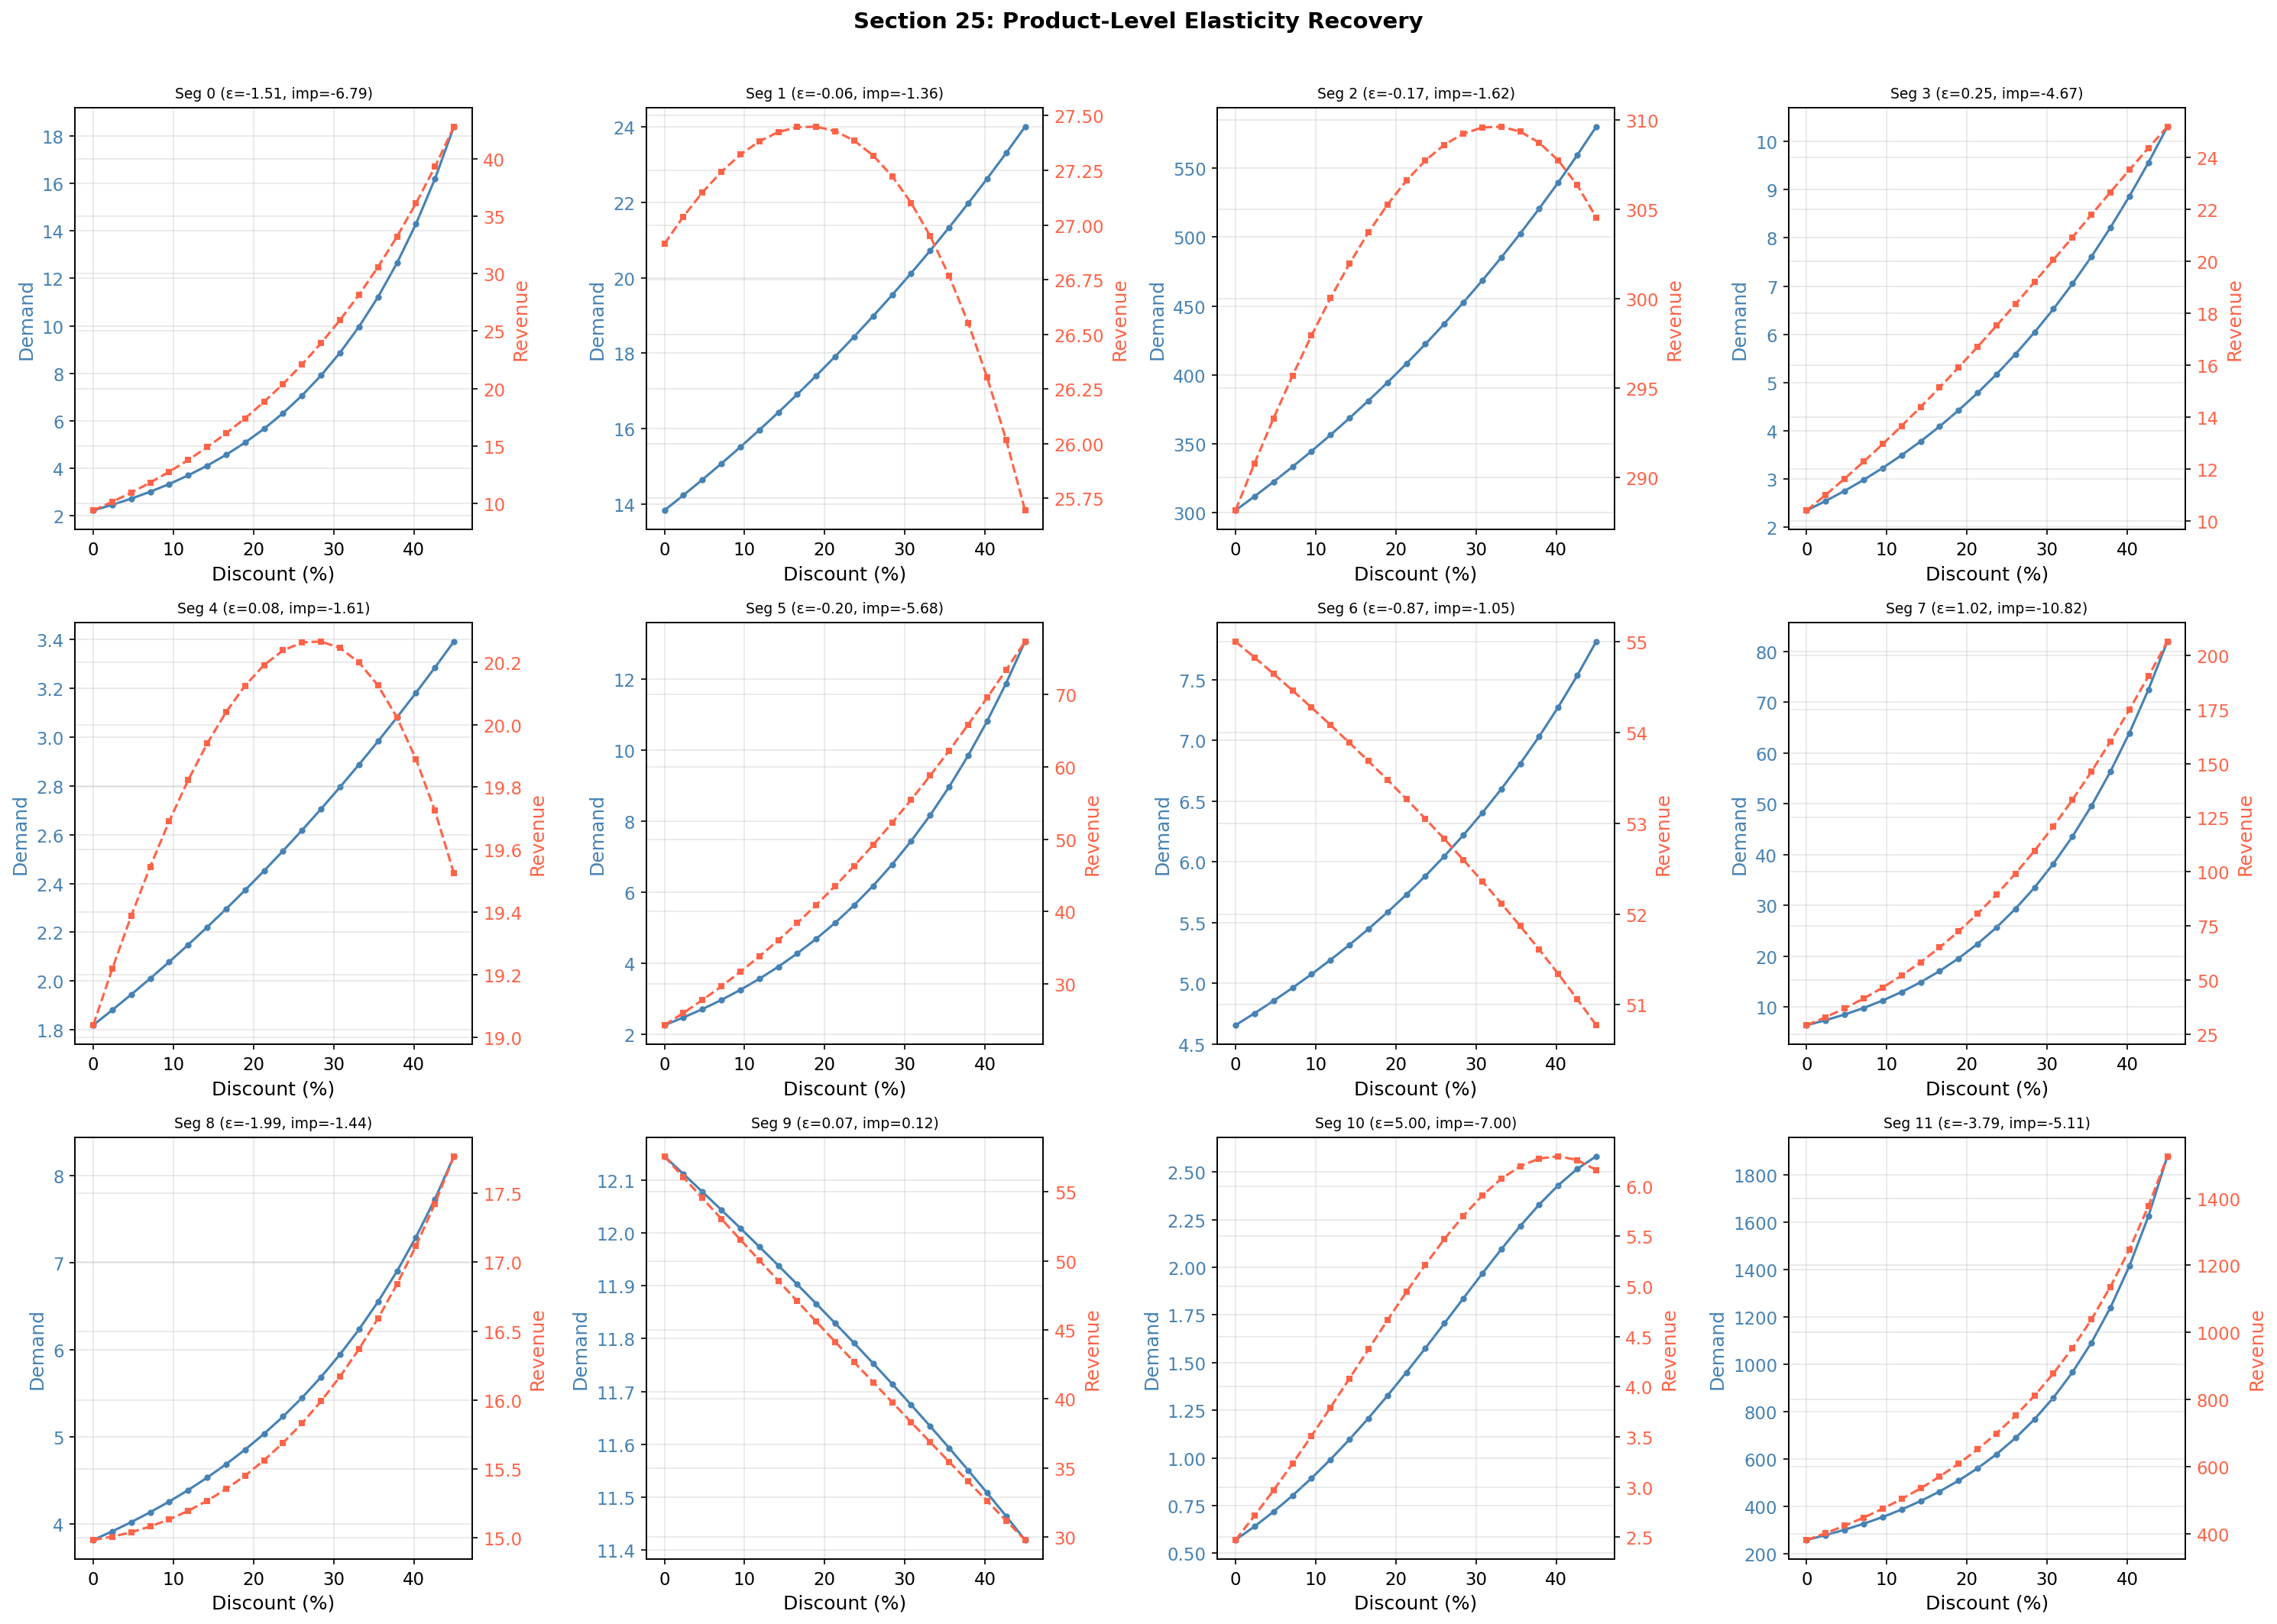
\includegraphics[width=\textwidth]{figures/21_elasticity_recovery_product.png}
\caption{Distribution of shrunk elasticities by segment, showing
substantial heterogeneity even within segments.}
\label{fig:elasticity-recovery}
\end{figure}

%% ═══════════════════════════════════════════════════════════
\section{Discussion}
\label{sec:discussion}
%% ═══════════════════════════════════════════════════════════

\subsection{Methodological Contributions}

\begin{enumerate}[nosep]
\item \textbf{Proper demand specification.} We identify and correct
a common error in markdown simulators where the discount effect is
double-counted by computing an ``effective price'' and feeding it
to the price elasticity coefficient. When the demand model is
estimated with shelf price and discount depth as separate
regressors, the simulator must use the shelf price (fixed) for
the elasticity term and the discount depth (variable) for the
promotional effect term.

\item \textbf{AR(1) demand persistence.} The lagged log-demand term
$\hat{\rho}_i \ln Q_{i,t-1}$ makes the simulator's demand
transition genuinely dynamic: the state variable $q_t$ now causally
influences the next-period demand, not just observationally. This
addresses the ``memoryless transitions'' criticism---the simulator's
demand process is no longer a repeated static response but an
autoregressive process where demand shocks persist over time.

\item \textbf{Within-segment cross-product substitution.} The
substitution term $\hat{\lambda}_i \overline{d}_{-i,s(i),t}$
captures promotional cannibalization: when competitors in the same
segment are discounted, own demand falls. This means the simulator no
longer treats products independently---the discount decision for
one product affects demand for others, which is critical for
realistic policy evaluation of broad vs.\ targeted promotions.

\item \textbf{Stratified representative selection.} Revenue-tercile
stratified sampling (50\% top, 30\% middle, 20\% bottom) within
each segment ensures the selected products span the full revenue
distribution, rather than being dominated by head SKUs. This
reduces head-SKU selection bias and produces more representative
estimates of the full product assortment's promotional response.

\item \textbf{Full discount accounting.} All three discount
components in the Dunnhumby data (retail discount, coupon discount,
and coupon-match discount) are included in both the reconstructed
shelf price and the discount depth, ensuring consistent price
measurement across the estimation and simulation stages.

\item \textbf{Continuous promotional intensity.} By using the
continuous store-fraction of display and mailer exposure rather
than binary indicators, the demand model captures the intensity
dimension of promotional activity. A product displayed in 10\%
of stores receives a proportionally smaller estimated effect than
one displayed in all stores.

\item \textbf{Seasonality in the simulator.} The simulator includes
calendar-aware demand variation via cosine/sine Fourier terms
entered as deviations from training-period means. This allows the
simulator to evaluate whether promotions deployed early vs.\ late
in a seasonal cycle produce different revenue outcomes.

\item \textbf{Parameter-specific shrinkage.} The James--Stein
shrinkage weights use HC1 standard errors for each parameter rather
than a generic residual-variance proxy, aligning the degree of
regularization with the actual estimation uncertainty for each
coefficient.

\item \textbf{Comprehensive shrinkage scope.} All six slope
parameters (elasticity, discount effect, persistence, substitution,
display, and mailer) are shrunk toward segment medians, with
post-shrinkage sign constraints for economic consistency.
\end{enumerate}

\subsection{Limitations}

\begin{enumerate}[nosep]
\item \textbf{Limited demand persistence.} The AR(1) lagged-demand
term captures first-order demand ``stickiness'' (mean shrunk
$\hat\rho = 0.039$, 64/150 products nonzero), making transitions
no longer memoryless. However, the model does not capture richer
intertemporal dynamics such as stockpiling, post-promotion dips,
habituation, or reference-price adaptation. These would require
higher-order autoregressive terms, regime-switching, or structural
models of consumer inventory behaviour.

\item \textbf{Linear substitution.} The within-segment substitution
term captures first-order cannibalization via the mean discount
depth of segment competitors (mean shrunk $\hat\lambda = -0.852$,
80/150 products nonzero). However, the deviation-from-mean
specification is linear and symmetric. Non-linear patterns
(e.g., asymmetric cannibalization where premium products steal
share from economy products more than vice versa), cross-segment
substitution, and complementarity effects remain outside the model's
scope.

\item \textbf{Stratified sampling limitations.} The 150
representative products are selected via stratified
revenue-tercile sampling (50\% top / 30\% middle / 20\% bottom
within each segment), which ensures coverage across the revenue
distribution but is not random sampling. The results should be
interpreted as characterizing a commercially diverse subset of
the assortment, not the full product catalog.

\item \textbf{Endogeneity.} Price and discount decisions are made by
the retailer based on (partially) observed demand signals. Without
instrumental variables, the elasticity estimates suffer from
simultaneity bias. We partially mitigate this by separating
shelf-price elasticity from promotional discount effects.

\item \textbf{Elasticity attenuation.} The median shrunk elasticity
of $-0.215$ is an order of magnitude below the meta-analytic
literature mean of $-2.62$ (Bijmolt et~al.\ 2005). The remaining
attenuation toward zero is a known consequence of limited
shelf-price variation in the data and the non-positivity constraint.

\item \textbf{ML models not structurally comparable.} The tree-based
and neural network benchmarks are trained as flexible predictors
and then collapsed to two-parameter log-linear approximations via
finite differences for simulator integration. This is not equivalent
to simulating the original ML model. The selection of OLS for the
simulator is a structural compatibility decision, not solely a
performance comparison.

\item \textbf{Post-shrinkage constraints are modeling choices.}
Winsorization at the 2.5th/97.5th percentiles, the non-positivity
constraint on elasticities, the $[0,\,0.95]$ stationarity constraint
on persistence, and the non-positivity constraint on substitution
are ex~post structural edits that make the simulator stable for
optimization, but less faithful as a pure measurement device.

\item \textbf{Independent promotional noise.} Display and mailer
events are drawn independently of the retailer's discount decision.
In practice, the retailer jointly decides on discounts and
promotional support (display, mailer), which creates
selection effects that our model does not capture.
\end{enumerate}

%% ═══════════════════════════════════════════════════════════
\section{Conclusion}
\label{sec:conclusion}
%% ═══════════════════════════════════════════════════════════

We have developed a calibrated product-level promotion response
simulator that:

\begin{enumerate}[nosep]
\item Estimates demand at the individual SKU level using log-linear
models with continuous promotional controls (display fraction,
mailer fraction), seasonality, AR(1) demand persistence, and
within-segment cross-product substitution, achieving 46.1\%
out-of-sample MAPE and 0.694 lift correlation.

\item Properly separates shelf-price elasticity from promotional
discount effects in the simulator demand specification, avoiding
the common double-counting error.

\item Applies James--Stein empirical Bayes shrinkage with
parameter-specific standard errors and post-shrinkage constraints
to produce stable demand parameters for 150 representative
products (selected via stratified revenue-tercile sampling) from
11 segments, shrinking six coefficients---elasticity, discount
effect, display effect, mailer effect, demand persistence, and
substitution effect---toward segment medians.

\item Incorporates calendar-aware seasonality and stochastic
promotional events (display and mailer draws from truncated normal
distributions) as deviations from training-period means, enabling
evaluation of temporally varying promotion strategies.

\item Identifies targeted discount strategies that improve revenue by
up to 41.3\% over the no-discount baseline, with Monte Carlo
confidence intervals confirming result robustness.

\item Reveals that 64.7\% of products benefit from discounting, with
a median revenue uplift of 105.1\% (IQR: 36.8\%--288.8\%),
but the optimal discount depth varies substantially across products
and segments---motivating product-level rather than category-level
markdown decisions.
\end{enumerate}

The simulator captures own-product promotional response enriched by
first-order demand persistence and within-segment substitution under
budget constraints. It can serve as the foundation for reinforcement
learning or dynamic programming approaches to optimal discount
scheduling. Extensions to higher-order intertemporal dynamics
(stockpiling, post-promotion dips, reference-price effects),
cross-segment substitution, and joint discount-display optimization
remain important directions for future work.

%% ═══════════════════════════════════════════════════════════
\section*{References}
%% ═══════════════════════════════════════════════════════════

\begin{enumerate}[label={[\arabic*]}, nosep, leftmargin=*]
\item Ban, G.-Y.\ and Rudin, C.\ (2019). ``The Big Data Newsvendor:
Practical Insights from Machine Learning.'' \textit{Operations
Research}, 67(1), 90--108.

\item Bijmolt, T.H.A., van Heerde, H.J., and Pieters, R.G.M.\
(2005). ``New Empirical Generalizations on the Determinants of Price
Elasticity.'' \textit{Journal of Marketing Research}, 42(2), 141--156.

\item Blattberg, R.C.\ and Neslin, S.A.\ (1990).
\textit{Sales Promotion: Concepts, Methods, and Strategies.}
Prentice Hall.

\item Breiman, L.\ (2001). ``Random Forests.''
\textit{Machine Learning}, 45(1), 5--32.

\item Chen, T.\ and Guestrin, C.\ (2016). ``XGBoost: A Scalable Tree
Boosting System.'' \textit{Proc.\ KDD}, 785--794.

\item Duan, N.\ (1983). ``Smearing Estimate: A Nonparametric
Retransformation Method.'' \textit{Journal of the American Statistical
Association}, 78(383), 605--610.

\item Efron, B.\ and Morris, C.\ (1975). ``Data Analysis Using
Stein's Estimator and its Generalizations.'' \textit{Journal of the
American Statistical Association}, 70(350), 311--319.

\item Ferreira, K.J., Lee, B.H.A., and Simchi-Levi, D.\ (2016).
``Analytics for an Online Retailer: Demand Forecasting and Price
Optimization.'' \textit{Manufacturing \& Service Operations
Management}, 18(1), 69--88.

\item Ke, G.\ et~al.\ (2017). ``LightGBM: A Highly Efficient
Gradient Boosting Decision Tree.'' \textit{Advances in Neural
Information Processing Systems}, 30.

\item Phillips, R.L.\ (2005). \textit{Pricing and Revenue
Optimization.} Stanford University Press.

\item Talluri, K.T.\ and van Ryzin, G.J.\ (2004). \textit{The Theory
and Practice of Revenue Management.} Springer.

\item Tellis, G.J.\ (1988). ``The Price Elasticity of Selective
Demand: A Meta-Analysis of Econometric Models of Sales.''
\textit{Journal of Marketing Research}, 25(4), 331--341.

\item Van Heerde, H.J., Leeflang, P.S.H., and Wittink, D.R.\
(2004). ``Decomposing the Sales Promotion Bump with Store Data.''
\textit{Marketing Science}, 23(3), 317--334.
\end{enumerate}

\end{document}
